\documentclass[twoside]{book}

% Packages required by doxygen
\usepackage{fixltx2e}
\usepackage{calc}
\usepackage{doxygen}
\usepackage[export]{adjustbox} % also loads graphicx
\usepackage{graphicx}
\usepackage[utf8]{inputenc}
\usepackage{makeidx}
\usepackage{multicol}
\usepackage{multirow}
\PassOptionsToPackage{warn}{textcomp}
\usepackage{textcomp}
\usepackage[nointegrals]{wasysym}
\usepackage[table]{xcolor}

% Font selection
\usepackage[T1]{fontenc}
\usepackage[scaled=.90]{helvet}
\usepackage{courier}
\usepackage{amssymb}
\usepackage{sectsty}
\renewcommand{\familydefault}{\sfdefault}
\allsectionsfont{%
  \fontseries{bc}\selectfont%
  \color{darkgray}%
}
\renewcommand{\DoxyLabelFont}{%
  \fontseries{bc}\selectfont%
  \color{darkgray}%
}
\newcommand{\+}{\discretionary{\mbox{\scriptsize$\hookleftarrow$}}{}{}}

% Page & text layout
\usepackage{geometry}
\geometry{%
  a4paper,%
  top=2.5cm,%
  bottom=2.5cm,%
  left=2.5cm,%
  right=2.5cm%
}
\tolerance=750
\hfuzz=15pt
\hbadness=750
\setlength{\emergencystretch}{15pt}
\setlength{\parindent}{0cm}
\setlength{\parskip}{3ex plus 2ex minus 2ex}
\makeatletter
\renewcommand{\paragraph}{%
  \@startsection{paragraph}{4}{0ex}{-1.0ex}{1.0ex}{%
    \normalfont\normalsize\bfseries\SS@parafont%
  }%
}
\renewcommand{\subparagraph}{%
  \@startsection{subparagraph}{5}{0ex}{-1.0ex}{1.0ex}{%
    \normalfont\normalsize\bfseries\SS@subparafont%
  }%
}
\makeatother

% Headers & footers
\usepackage{fancyhdr}
\pagestyle{fancyplain}
\fancyhead[LE]{\fancyplain{}{\bfseries\thepage}}
\fancyhead[CE]{\fancyplain{}{}}
\fancyhead[RE]{\fancyplain{}{\bfseries\leftmark}}
\fancyhead[LO]{\fancyplain{}{\bfseries\rightmark}}
\fancyhead[CO]{\fancyplain{}{}}
\fancyhead[RO]{\fancyplain{}{\bfseries\thepage}}
\fancyfoot[LE]{\fancyplain{}{}}
\fancyfoot[CE]{\fancyplain{}{}}
\fancyfoot[RE]{\fancyplain{}{\bfseries\scriptsize Generated by Doxygen }}
\fancyfoot[LO]{\fancyplain{}{\bfseries\scriptsize Generated by Doxygen }}
\fancyfoot[CO]{\fancyplain{}{}}
\fancyfoot[RO]{\fancyplain{}{}}
\renewcommand{\footrulewidth}{0.4pt}
\renewcommand{\chaptermark}[1]{%
  \markboth{#1}{}%
}
\renewcommand{\sectionmark}[1]{%
  \markright{\thesection\ #1}%
}

% Indices & bibliography
\usepackage{natbib}
\usepackage[titles]{tocloft}
\setcounter{tocdepth}{3}
\setcounter{secnumdepth}{5}
\makeindex

% Hyperlinks (required, but should be loaded last)
\usepackage{ifpdf}
\ifpdf
  \usepackage[pdftex,pagebackref=true]{hyperref}
\else
  \usepackage[ps2pdf,pagebackref=true]{hyperref}
\fi
\hypersetup{%
  colorlinks=true,%
  linkcolor=blue,%
  citecolor=blue,%
  unicode%
}

% Custom commands
\newcommand{\clearemptydoublepage}{%
  \newpage{\pagestyle{empty}\cleardoublepage}%
}

\usepackage{caption}
\captionsetup{labelsep=space,justification=centering,font={bf},singlelinecheck=off,skip=4pt,position=top}

%===== C O N T E N T S =====

\begin{document}

% Titlepage & ToC
\hypersetup{pageanchor=false,
             bookmarksnumbered=true,
             pdfencoding=unicode
            }
\pagenumbering{alph}
\begin{titlepage}
\vspace*{7cm}
\begin{center}%
{\Large Beer\+Game }\\
\vspace*{1cm}
{\large Generated by Doxygen 1.8.13}\\
\end{center}
\end{titlepage}
\clearemptydoublepage
\pagenumbering{roman}
\tableofcontents
\clearemptydoublepage
\pagenumbering{arabic}
\hypersetup{pageanchor=true}

%--- Begin generated contents ---
\chapter{se-\/02-\/team-\/24}
\label{md__home_kinky_tail_se-02-team-24__r_e_a_d_m_e}
\Hypertarget{md__home_kinky_tail_se-02-team-24__r_e_a_d_m_e}
\input{md__home_kinky_tail_se-02-team-24__r_e_a_d_m_e}
\chapter{Namespace Index}
\section{Namespace List}
Here is a list of all namespaces with brief descriptions\+:\begin{DoxyCompactList}
\item\contentsline{section}{\hyperlink{namespace_ui}{Ui} }{\pageref{namespace_ui}}{}
\end{DoxyCompactList}

\chapter{Hierarchical Index}
\section{Class Hierarchy}
This inheritance list is sorted roughly, but not completely, alphabetically\+:\begin{DoxyCompactList}
\item \contentsline{section}{Game}{\pageref{class_game}}{}
\item \contentsline{section}{Instructor}{\pageref{class_instructor}}{}
\item \contentsline{section}{Order}{\pageref{class_order}}{}
\item \contentsline{section}{Player}{\pageref{class_player}}{}
\begin{DoxyCompactList}
\item \contentsline{section}{Factory}{\pageref{class_factory}}{}
\end{DoxyCompactList}
\item Q\+Main\+Window\begin{DoxyCompactList}
\item \contentsline{section}{Main\+Window}{\pageref{class_main_window}}{}
\end{DoxyCompactList}
\end{DoxyCompactList}

\chapter{Class Index}
\section{Class List}
Here are the classes, structs, unions and interfaces with brief descriptions\+:\begin{DoxyCompactList}
\item\contentsline{section}{\hyperlink{class_factory}{Factory} }{\pageref{class_factory}}{}
\item\contentsline{section}{\hyperlink{class_game}{Game} }{\pageref{class_game}}{}
\item\contentsline{section}{\hyperlink{class_instructor}{Instructor} }{\pageref{class_instructor}}{}
\item\contentsline{section}{\hyperlink{class_main_window}{Main\+Window} }{\pageref{class_main_window}}{}
\item\contentsline{section}{\hyperlink{class_order}{Order} }{\pageref{class_order}}{}
\item\contentsline{section}{\hyperlink{class_player}{Player} }{\pageref{class_player}}{}
\end{DoxyCompactList}

\chapter{File Index}
\section{File List}
Here is a list of all files with brief descriptions\+:\begin{DoxyCompactList}
\item\contentsline{section}{/home/kinky\+\_\+tail/se-\/02-\/team-\/24/src/\hyperlink{factory_8cpp}{factory.\+cpp} }{\pageref{factory_8cpp}}{}
\item\contentsline{section}{/home/kinky\+\_\+tail/se-\/02-\/team-\/24/src/\hyperlink{factory_8h}{factory.\+h} }{\pageref{factory_8h}}{}
\item\contentsline{section}{/home/kinky\+\_\+tail/se-\/02-\/team-\/24/src/\hyperlink{game_8cpp}{game.\+cpp} }{\pageref{game_8cpp}}{}
\item\contentsline{section}{/home/kinky\+\_\+tail/se-\/02-\/team-\/24/src/\hyperlink{game_8h}{game.\+h} }{\pageref{game_8h}}{}
\item\contentsline{section}{/home/kinky\+\_\+tail/se-\/02-\/team-\/24/src/\hyperlink{instructor_8cpp}{instructor.\+cpp} }{\pageref{instructor_8cpp}}{}
\item\contentsline{section}{/home/kinky\+\_\+tail/se-\/02-\/team-\/24/src/\hyperlink{instructor_8h}{instructor.\+h} }{\pageref{instructor_8h}}{}
\item\contentsline{section}{/home/kinky\+\_\+tail/se-\/02-\/team-\/24/src/\hyperlink{main_8cpp}{main.\+cpp} }{\pageref{main_8cpp}}{}
\item\contentsline{section}{/home/kinky\+\_\+tail/se-\/02-\/team-\/24/src/\hyperlink{mainwindow_8cpp}{mainwindow.\+cpp} }{\pageref{mainwindow_8cpp}}{}
\item\contentsline{section}{/home/kinky\+\_\+tail/se-\/02-\/team-\/24/src/\hyperlink{mainwindow_8h}{mainwindow.\+h} }{\pageref{mainwindow_8h}}{}
\item\contentsline{section}{/home/kinky\+\_\+tail/se-\/02-\/team-\/24/src/\hyperlink{order_8cpp}{order.\+cpp} }{\pageref{order_8cpp}}{}
\item\contentsline{section}{/home/kinky\+\_\+tail/se-\/02-\/team-\/24/src/\hyperlink{order_8h}{order.\+h} }{\pageref{order_8h}}{}
\item\contentsline{section}{/home/kinky\+\_\+tail/se-\/02-\/team-\/24/src/\hyperlink{player_8cpp}{player.\+cpp} }{\pageref{player_8cpp}}{}
\item\contentsline{section}{/home/kinky\+\_\+tail/se-\/02-\/team-\/24/src/\hyperlink{player_8h}{player.\+h} }{\pageref{player_8h}}{}
\end{DoxyCompactList}

\chapter{Namespace Documentation}
\hypertarget{namespace_ui}{}\section{Ui Namespace Reference}
\label{namespace_ui}\index{Ui@{Ui}}

\chapter{Class Documentation}
\hypertarget{class_factory}{}\section{Factory Class Reference}
\label{class_factory}\index{Factory@{Factory}}


{\ttfamily \#include $<$factory.\+h$>$}

Inheritance diagram for Factory\+:\begin{figure}[H]
\begin{center}
\leavevmode
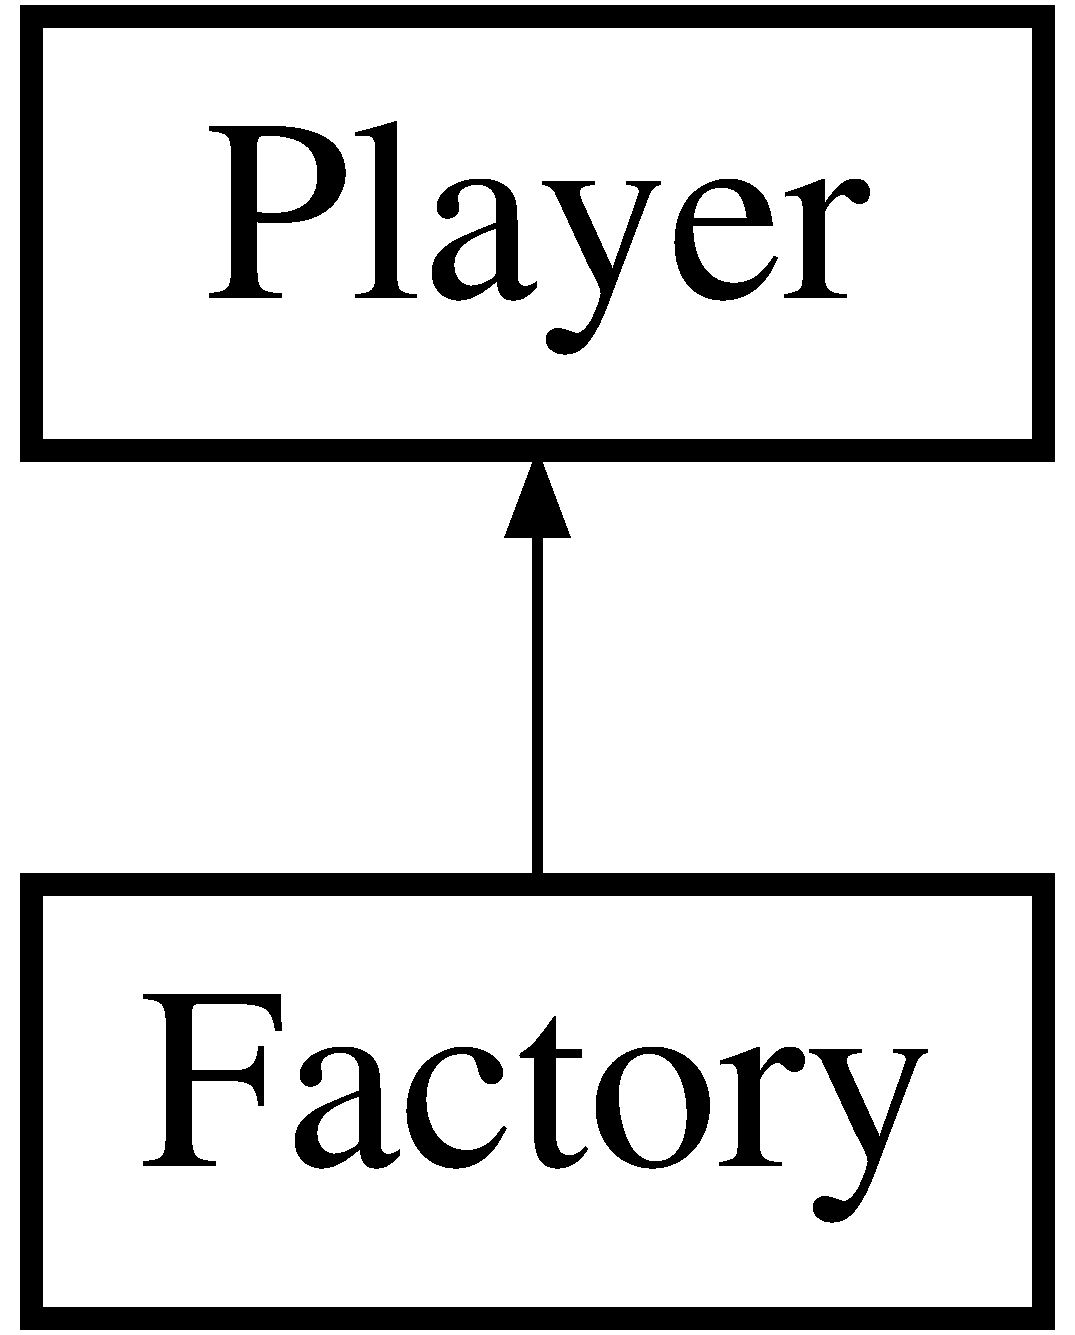
\includegraphics[height=2.000000cm]{class_factory}
\end{center}
\end{figure}
\subsection*{Public Member Functions}
\begin{DoxyCompactItemize}
\item 
\hyperlink{class_factory_ac792bf88cfb7b6804b479529da5308cc}{Factory} ()
\begin{DoxyCompactList}\small\item\em Constructor for game class, sets the default values for game class. \end{DoxyCompactList}\item 
\hyperlink{class_factory_a8f71456f48e4df402c778a44191ff40e}{$\sim$\+Factory} ()
\begin{DoxyCompactList}\small\item\em distructor for game class \end{DoxyCompactList}\item 
void \hyperlink{class_factory_a8567550501860453df05d6afae963997}{set\+Production\+Time} (int value)
\begin{DoxyCompactList}\small\item\em Setter method for production delay. \end{DoxyCompactList}\item 
int \hyperlink{class_factory_a7020f06a3b9045d0902cd3740796ded5}{get\+Production\+Time} () const
\begin{DoxyCompactList}\small\item\em Getter method for Production time. \end{DoxyCompactList}\item 
void \hyperlink{class_factory_a321703fafe2a870260e04b848aa565d2}{produce} (int n)
\begin{DoxyCompactList}\small\item\em Attribute for describing number of beers to be produced. \end{DoxyCompactList}\end{DoxyCompactItemize}
\subsection*{Private Attributes}
\begin{DoxyCompactItemize}
\item 
int \hyperlink{class_factory_ab3a36b3ceb997d9e3fcc534c45fef354}{production\+Time}
\begin{DoxyCompactList}\small\item\em Attribute for Production Time. \end{DoxyCompactList}\end{DoxyCompactItemize}


\subsection{Constructor \& Destructor Documentation}
\mbox{\Hypertarget{class_factory_ac792bf88cfb7b6804b479529da5308cc}\label{class_factory_ac792bf88cfb7b6804b479529da5308cc}} 
\index{Factory@{Factory}!Factory@{Factory}}
\index{Factory@{Factory}!Factory@{Factory}}
\subsubsection{\texorpdfstring{Factory()}{Factory()}}
{\footnotesize\ttfamily Factory\+::\+Factory (\begin{DoxyParamCaption}{ }\end{DoxyParamCaption})}



Constructor for game class, sets the default values for game class. 

\mbox{\Hypertarget{class_factory_a8f71456f48e4df402c778a44191ff40e}\label{class_factory_a8f71456f48e4df402c778a44191ff40e}} 
\index{Factory@{Factory}!````~Factory@{$\sim$\+Factory}}
\index{````~Factory@{$\sim$\+Factory}!Factory@{Factory}}
\subsubsection{\texorpdfstring{$\sim$\+Factory()}{~Factory()}}
{\footnotesize\ttfamily Factory\+::$\sim$\+Factory (\begin{DoxyParamCaption}{ }\end{DoxyParamCaption})}



distructor for game class 



\subsection{Member Function Documentation}
\mbox{\Hypertarget{class_factory_a7020f06a3b9045d0902cd3740796ded5}\label{class_factory_a7020f06a3b9045d0902cd3740796ded5}} 
\index{Factory@{Factory}!get\+Production\+Time@{get\+Production\+Time}}
\index{get\+Production\+Time@{get\+Production\+Time}!Factory@{Factory}}
\subsubsection{\texorpdfstring{get\+Production\+Time()}{getProductionTime()}}
{\footnotesize\ttfamily int Factory\+::get\+Production\+Time (\begin{DoxyParamCaption}{ }\end{DoxyParamCaption}) const}



Getter method for Production time. 

\begin{DoxyReturn}{Returns}
production time 
\end{DoxyReturn}
\mbox{\Hypertarget{class_factory_a321703fafe2a870260e04b848aa565d2}\label{class_factory_a321703fafe2a870260e04b848aa565d2}} 
\index{Factory@{Factory}!produce@{produce}}
\index{produce@{produce}!Factory@{Factory}}
\subsubsection{\texorpdfstring{produce()}{produce()}}
{\footnotesize\ttfamily void Factory\+::produce (\begin{DoxyParamCaption}\item[{int}]{n }\end{DoxyParamCaption})}



Attribute for describing number of beers to be produced. 

\mbox{\Hypertarget{class_factory_a8567550501860453df05d6afae963997}\label{class_factory_a8567550501860453df05d6afae963997}} 
\index{Factory@{Factory}!set\+Production\+Time@{set\+Production\+Time}}
\index{set\+Production\+Time@{set\+Production\+Time}!Factory@{Factory}}
\subsubsection{\texorpdfstring{set\+Production\+Time()}{setProductionTime()}}
{\footnotesize\ttfamily void Factory\+::set\+Production\+Time (\begin{DoxyParamCaption}\item[{int}]{value }\end{DoxyParamCaption})}



Setter method for production delay. 


\begin{DoxyParams}{Parameters}
{\em n} & seeting value for the order delay \\
\hline
\end{DoxyParams}


\subsection{Member Data Documentation}
\mbox{\Hypertarget{class_factory_ab3a36b3ceb997d9e3fcc534c45fef354}\label{class_factory_ab3a36b3ceb997d9e3fcc534c45fef354}} 
\index{Factory@{Factory}!production\+Time@{production\+Time}}
\index{production\+Time@{production\+Time}!Factory@{Factory}}
\subsubsection{\texorpdfstring{production\+Time}{productionTime}}
{\footnotesize\ttfamily int Factory\+::production\+Time\hspace{0.3cm}{\ttfamily [private]}}



Attribute for Production Time. 



The documentation for this class was generated from the following files\+:\begin{DoxyCompactItemize}
\item 
/home/kinky\+\_\+tail/se-\/02-\/team-\/24/src/\hyperlink{factory_8h}{factory.\+h}\item 
/home/kinky\+\_\+tail/se-\/02-\/team-\/24/src/\hyperlink{factory_8cpp}{factory.\+cpp}\end{DoxyCompactItemize}

\hypertarget{class_game}{}\section{Game Class Reference}
\label{class_game}\index{Game@{Game}}


{\ttfamily \#include $<$game.\+h$>$}

\subsection*{Public Member Functions}
\begin{DoxyCompactItemize}
\item 
\hyperlink{class_game_ad59df6562a58a614fda24622d3715b65}{Game} ()
\begin{DoxyCompactList}\small\item\em Constructor for game class, sets the default values for game class. \end{DoxyCompactList}\item 
\hyperlink{class_game_ae3d112ca6e0e55150d2fdbc704474530}{$\sim$\+Game} ()
\begin{DoxyCompactList}\small\item\em distructor for game class \end{DoxyCompactList}\item 
int \hyperlink{class_game_aa48501c52deee3c167334844e72a16b9}{execute\+Orders\+For\+Current\+Week} ()
\begin{DoxyCompactList}\small\item\em Method to execute orders for current week. \end{DoxyCompactList}\item 
int \hyperlink{class_game_a87b96a8975a2db552b1f556f488211c3}{update\+Player\+Inventories} ()
\begin{DoxyCompactList}\small\item\em Method to update player inventories. \end{DoxyCompactList}\item 
int \hyperlink{class_game_a8471ea91ed18fc2d289eb23747d11d39}{advance\+Week} ()
\begin{DoxyCompactList}\small\item\em Method advance a week during the game. \end{DoxyCompactList}\item 
void \hyperlink{class_game_a0e6b1f8c9d598c7eb860d04c218fa546}{add\+Order} (\hyperlink{class_order}{Order} order)
\begin{DoxyCompactList}\small\item\em Method to add order. \end{DoxyCompactList}\item 
std\+::vector$<$ std\+::string $>$ \hyperlink{class_game_aa083541e01feec6694497e8c6eb5ffe8}{generate\+Passwords} (int n)
\begin{DoxyCompactList}\small\item\em Method to generate passwords for player in the game. \end{DoxyCompactList}\item 
void \hyperlink{class_game_a4216dd9e4b966f68cebcd4914a203edb}{set\+G\+Id} (int n\+\_\+id)
\begin{DoxyCompactList}\small\item\em Setter method for the \hyperlink{class_game}{Game} Id. \end{DoxyCompactList}\item 
void \hyperlink{class_game_a7a704228c549b80d48d1b4fb5a8dd512}{set\+Instr\+Id} (int n\+\_\+id)
\begin{DoxyCompactList}\small\item\em Setter method for the \hyperlink{class_instructor}{Instructor} Id. \end{DoxyCompactList}\item 
void \hyperlink{class_game_a727c19b36849f11e1e08d05af9162388}{set\+P\+Fact\+Id} (int n\+\_\+id)
\begin{DoxyCompactList}\small\item\em Setter method for the \hyperlink{class_factory}{Factory} Id. \end{DoxyCompactList}\item 
void \hyperlink{class_game_a98cdfae7d20ad4c4f7a34ed56e64ab7c}{set\+P\+Distributor\+Id} (int n\+\_\+id)
\begin{DoxyCompactList}\small\item\em Setter method for the Distributor Id. \end{DoxyCompactList}\item 
void \hyperlink{class_game_a945968b2490656de58ce89b653eb30e8}{set\+P\+Wholesaler\+Id} (int n\+\_\+id)
\begin{DoxyCompactList}\small\item\em Setter method for the Wholesaler Id. \end{DoxyCompactList}\item 
void \hyperlink{class_game_a80b5a91e9262403dfac82f961056c79a}{set\+P\+Retailer\+Id} (int n\+\_\+id)
\begin{DoxyCompactList}\small\item\em Setter method for the Retailer Id. \end{DoxyCompactList}\item 
void \hyperlink{class_game_af127a9a8e81e7863d6cb73025181a62b}{set\+Order\+Time\+Delay} (int n)
\begin{DoxyCompactList}\small\item\em Setter method for the \hyperlink{class_order}{Order} Time delay. \end{DoxyCompactList}\item 
void \hyperlink{class_game_abae5ec4f77327efde1516e8bd1edda2b}{set\+Weeks\+To\+Be\+Played} (int n)
\begin{DoxyCompactList}\small\item\em Setter method for Weeks to be played. \end{DoxyCompactList}\item 
void \hyperlink{class_game_a8da75fddaf91545459de45a52f604ebb}{set\+Info\+Code} (int n)
\begin{DoxyCompactList}\small\item\em Setter method for the Info code. \end{DoxyCompactList}\item 
void \hyperlink{class_game_a5136cc3fd07b605ed6df658024eb1e88}{set\+Holding\+Cost} (double n)
\begin{DoxyCompactList}\small\item\em Setter method for the Holding cost. \end{DoxyCompactList}\item 
void \hyperlink{class_game_aa994becb6fe955b2ed8dad3a24a57937}{set\+Starting\+Inventory} (int n)
\begin{DoxyCompactList}\small\item\em Setter method for the Starting inventory. \end{DoxyCompactList}\item 
void \hyperlink{class_game_a6526b895b01b619358918e5276314f43}{set\+Backorder\+Cost} (double n)
\begin{DoxyCompactList}\small\item\em Setter method for Backorder cost. \end{DoxyCompactList}\item 
void \hyperlink{class_game_a5d7966304ef0340bc9c1586bcee55738}{set\+Current\+Week} (int n)
\begin{DoxyCompactList}\small\item\em Setter method for the Current Week. \end{DoxyCompactList}\item 
void \hyperlink{class_game_adf895b54f74b8d95c4f67b15cef75290}{set\+Order\+Delay} (int n)
\begin{DoxyCompactList}\small\item\em Setter method for the \hyperlink{class_order}{Order} delay. \end{DoxyCompactList}\item 
void \hyperlink{class_game_a1b45bb18641fd7b60c2b887899fe4464}{set\+Shipment\+Delay} (int n)
\begin{DoxyCompactList}\small\item\em Setter method for the Shipment delay. \end{DoxyCompactList}\item 
int \hyperlink{class_game_aea578dd12fcdf404231a14ecc18fb98a}{get\+G\+Id} ()
\begin{DoxyCompactList}\small\item\em Getter method for \hyperlink{class_game}{Game} Id. \end{DoxyCompactList}\item 
int \hyperlink{class_game_a52dd61290996a492087b81464eba52c8}{get\+Instr\+Id} ()
\begin{DoxyCompactList}\small\item\em Getter method for instructor Id. \end{DoxyCompactList}\item 
int \hyperlink{class_game_a9d4b2445fa34422a03d99edba54c0c28}{get\+P\+Fact\+Id} ()
\begin{DoxyCompactList}\small\item\em Getter method for \hyperlink{class_factory}{Factory} Id. \end{DoxyCompactList}\item 
int \hyperlink{class_game_ab59b422a861f1aa2d59c176b9b57ed80}{get\+P\+Distributor\+Id} ()
\begin{DoxyCompactList}\small\item\em Getter method for distributor Id. \end{DoxyCompactList}\item 
int \hyperlink{class_game_a7a93d4a8c499ee090efd397fc068a3c4}{get\+P\+Wholesaler\+Id} ()
\begin{DoxyCompactList}\small\item\em Getter method for wholeseller Id. \end{DoxyCompactList}\item 
int \hyperlink{class_game_ac8cb0ad6c01ecddc3c76bb0bdbc9202b}{get\+P\+Retailer\+Id} ()
\begin{DoxyCompactList}\small\item\em Getter method for retailer Id. \end{DoxyCompactList}\item 
int \hyperlink{class_game_a61aed9159fe6130486be8034f3e28086}{get\+Order\+Time\+Delay} ()
\begin{DoxyCompactList}\small\item\em Getter method for \hyperlink{class_order}{Order} Time dealy. \end{DoxyCompactList}\item 
int \hyperlink{class_game_ad9d402aa7fdf97b4cbfa9e8e04301da0}{get\+Weeks\+To\+Be\+Played} ()
\begin{DoxyCompactList}\small\item\em Getter method for weeks to be played. \end{DoxyCompactList}\item 
int \hyperlink{class_game_a16cbdc46bd7268319249affa2f24ef3a}{get\+Info\+Code} ()
\begin{DoxyCompactList}\small\item\em Getter method for Info Code. \end{DoxyCompactList}\item 
double \hyperlink{class_game_a7bba0862ffb4fc160a491c982f70a113}{get\+Holding\+Cost} ()
\begin{DoxyCompactList}\small\item\em Getter method for Holding cost. \end{DoxyCompactList}\item 
int \hyperlink{class_game_aab81a9ebaccae9567297d73a44204e0d}{get\+Starting\+Inventory} ()
\begin{DoxyCompactList}\small\item\em Getter method for Starting Inventory. \end{DoxyCompactList}\item 
double \hyperlink{class_game_ab29ec1e3f5dd71e0f67b3bda884ff166}{get\+Backorder\+Cost} ()
\begin{DoxyCompactList}\small\item\em Getter method for Backorder Cost. \end{DoxyCompactList}\item 
int \hyperlink{class_game_aa131c51d4b09434ec8986048483ef17e}{get\+Current\+Week} ()
\begin{DoxyCompactList}\small\item\em Getter method for current cost. \end{DoxyCompactList}\item 
int \hyperlink{class_game_ab8a2d3843e55b53345bdb80b6b1e6503}{get\+Order\+Delay} ()
\begin{DoxyCompactList}\small\item\em Getter method for \hyperlink{class_order}{Order} delay. \end{DoxyCompactList}\item 
int \hyperlink{class_game_a9e3acf4f2ee399be2eb047ed036bc24f}{get\+Shipment\+Delay} ()
\begin{DoxyCompactList}\small\item\em Getter method for Shipment delay. \end{DoxyCompactList}\end{DoxyCompactItemize}
\subsection*{Private Attributes}
\begin{DoxyCompactItemize}
\item 
int \hyperlink{class_game_a448cd197d12e3051ca3946906917eb97}{g\+Id}
\begin{DoxyCompactList}\small\item\em Attribute for \hyperlink{class_game}{Game} Id. \end{DoxyCompactList}\item 
int \hyperlink{class_game_ad12306e232a5ed72de6435c77383cfe2}{Instr\+Id}
\begin{DoxyCompactList}\small\item\em Attribute for \hyperlink{class_instructor}{Instructor} Id. \end{DoxyCompactList}\item 
int \hyperlink{class_game_ac516a7154e48c4ca10b40da5c1a1ab6d}{p\+Fact\+Id}
\begin{DoxyCompactList}\small\item\em Attribute for \hyperlink{class_factory}{Factory} Id. \end{DoxyCompactList}\item 
int \hyperlink{class_game_a3a1c85c5fdd16e9b99ba4c45ae2c6368}{p\+Distributor\+Id}
\begin{DoxyCompactList}\small\item\em Attribute for Distributor Id. \end{DoxyCompactList}\item 
int \hyperlink{class_game_a3d318d2ddeeba939359c1c3bdf17e0eb}{p\+Wholeseller\+Id}
\begin{DoxyCompactList}\small\item\em Attribute for Wholeseller Id. \end{DoxyCompactList}\item 
int \hyperlink{class_game_aad086ef718ee39a0b0f72fbfafb5e30c}{p\+Retailer\+Id}
\begin{DoxyCompactList}\small\item\em Attribute for Retailer Id. \end{DoxyCompactList}\item 
std\+::map$<$ int, std\+::vector$<$ \hyperlink{class_order}{Order} $>$ $>$ \hyperlink{class_game_ae48a7dd1eb19120b78b70d3814d207fc}{orders\+To\+Be\+Executed}
\begin{DoxyCompactList}\small\item\em Attribute which maps orders to orders to be executed vector. \end{DoxyCompactList}\item 
std\+::vector$<$ int $>$ \hyperlink{class_game_aea9436a9a1e01665fc10fed6e8273388}{demand\+Per\+Week}
\begin{DoxyCompactList}\small\item\em Attribute which defines the order for that week. \end{DoxyCompactList}\item 
int \hyperlink{class_game_a337c34aba5afe4984d5a76e2dfb8800e}{order\+Time\+Delay}
\begin{DoxyCompactList}\small\item\em Attribute for \hyperlink{class_order}{Order} time delay. \end{DoxyCompactList}\item 
double \hyperlink{class_game_a6cb7c7d62127e8378a0dda6793916efd}{holding\+Cost}
\begin{DoxyCompactList}\small\item\em Attribute for Holding cost for a game. \end{DoxyCompactList}\item 
double \hyperlink{class_game_a413dfabbdffaf493bca059932fe09701}{backorder\+Cost}
\begin{DoxyCompactList}\small\item\em Attribute for Back order cost for a game. \end{DoxyCompactList}\item 
int \hyperlink{class_game_a903867ea1af339a759f931a726b43f0e}{Starting\+Inventory}
\begin{DoxyCompactList}\small\item\em Attribute for Starting inventory. \end{DoxyCompactList}\item 
int \hyperlink{class_game_ab577818246babc5bbd94059d33553c70}{weeks\+To\+Be\+Played}
\begin{DoxyCompactList}\small\item\em Attribute to define total no of weeks the game is being played. \end{DoxyCompactList}\item 
int \hyperlink{class_game_a271387bda026cec90a6bb370ce74278d}{current\+Week}
\begin{DoxyCompactList}\small\item\em Attribute for Current week. \end{DoxyCompactList}\item 
int \hyperlink{class_game_ac8a93c181fc5a54ca38ad59c9bff25a0}{info\+Code}
\begin{DoxyCompactList}\small\item\em Attribute for info code. \end{DoxyCompactList}\item 
int \hyperlink{class_game_afc75f56db8dd8f3ffe78d670eeea536d}{order\+Delay}
\begin{DoxyCompactList}\small\item\em Attribute for \hyperlink{class_order}{Order} delay. \end{DoxyCompactList}\item 
int \hyperlink{class_game_ae7c8b91149db62d25ea552d71b053bde}{shipment\+Delay}
\begin{DoxyCompactList}\small\item\em Shipment delay of a specific game. \end{DoxyCompactList}\end{DoxyCompactItemize}


\subsection{Constructor \& Destructor Documentation}
\mbox{\Hypertarget{class_game_ad59df6562a58a614fda24622d3715b65}\label{class_game_ad59df6562a58a614fda24622d3715b65}} 
\index{Game@{Game}!Game@{Game}}
\index{Game@{Game}!Game@{Game}}
\subsubsection{\texorpdfstring{Game()}{Game()}}
{\footnotesize\ttfamily Game\+::\+Game (\begin{DoxyParamCaption}{ }\end{DoxyParamCaption})}



Constructor for game class, sets the default values for game class. 

\mbox{\Hypertarget{class_game_ae3d112ca6e0e55150d2fdbc704474530}\label{class_game_ae3d112ca6e0e55150d2fdbc704474530}} 
\index{Game@{Game}!````~Game@{$\sim$\+Game}}
\index{````~Game@{$\sim$\+Game}!Game@{Game}}
\subsubsection{\texorpdfstring{$\sim$\+Game()}{~Game()}}
{\footnotesize\ttfamily Game\+::$\sim$\+Game (\begin{DoxyParamCaption}{ }\end{DoxyParamCaption})}



distructor for game class 



\subsection{Member Function Documentation}
\mbox{\Hypertarget{class_game_a0e6b1f8c9d598c7eb860d04c218fa546}\label{class_game_a0e6b1f8c9d598c7eb860d04c218fa546}} 
\index{Game@{Game}!add\+Order@{add\+Order}}
\index{add\+Order@{add\+Order}!Game@{Game}}
\subsubsection{\texorpdfstring{add\+Order()}{addOrder()}}
{\footnotesize\ttfamily void Game\+::add\+Order (\begin{DoxyParamCaption}\item[{\hyperlink{class_order}{Order}}]{order }\end{DoxyParamCaption})}



Method to add order. 


\begin{DoxyParams}{Parameters}
{\em order} & is the order to be added \\
\hline
\end{DoxyParams}
\mbox{\Hypertarget{class_game_a8471ea91ed18fc2d289eb23747d11d39}\label{class_game_a8471ea91ed18fc2d289eb23747d11d39}} 
\index{Game@{Game}!advance\+Week@{advance\+Week}}
\index{advance\+Week@{advance\+Week}!Game@{Game}}
\subsubsection{\texorpdfstring{advance\+Week()}{advanceWeek()}}
{\footnotesize\ttfamily int Game\+::advance\+Week (\begin{DoxyParamCaption}{ }\end{DoxyParamCaption})}



Method advance a week during the game. 

\mbox{\Hypertarget{class_game_aa48501c52deee3c167334844e72a16b9}\label{class_game_aa48501c52deee3c167334844e72a16b9}} 
\index{Game@{Game}!execute\+Orders\+For\+Current\+Week@{execute\+Orders\+For\+Current\+Week}}
\index{execute\+Orders\+For\+Current\+Week@{execute\+Orders\+For\+Current\+Week}!Game@{Game}}
\subsubsection{\texorpdfstring{execute\+Orders\+For\+Current\+Week()}{executeOrdersForCurrentWeek()}}
{\footnotesize\ttfamily int Game\+::execute\+Orders\+For\+Current\+Week (\begin{DoxyParamCaption}{ }\end{DoxyParamCaption})}



Method to execute orders for current week. 

\mbox{\Hypertarget{class_game_aa083541e01feec6694497e8c6eb5ffe8}\label{class_game_aa083541e01feec6694497e8c6eb5ffe8}} 
\index{Game@{Game}!generate\+Passwords@{generate\+Passwords}}
\index{generate\+Passwords@{generate\+Passwords}!Game@{Game}}
\subsubsection{\texorpdfstring{generate\+Passwords()}{generatePasswords()}}
{\footnotesize\ttfamily std\+::vector$<$ std\+::string $>$ Game\+::generate\+Passwords (\begin{DoxyParamCaption}\item[{int}]{n }\end{DoxyParamCaption})}



Method to generate passwords for player in the game. 


\begin{DoxyParams}{Parameters}
{\em n} & describes the no of passwords to be generated \\
\hline
\end{DoxyParams}
\mbox{\Hypertarget{class_game_ab29ec1e3f5dd71e0f67b3bda884ff166}\label{class_game_ab29ec1e3f5dd71e0f67b3bda884ff166}} 
\index{Game@{Game}!get\+Backorder\+Cost@{get\+Backorder\+Cost}}
\index{get\+Backorder\+Cost@{get\+Backorder\+Cost}!Game@{Game}}
\subsubsection{\texorpdfstring{get\+Backorder\+Cost()}{getBackorderCost()}}
{\footnotesize\ttfamily double Game\+::get\+Backorder\+Cost (\begin{DoxyParamCaption}{ }\end{DoxyParamCaption})}



Getter method for Backorder Cost. 

\begin{DoxyReturn}{Returns}
Backorder Cost 
\end{DoxyReturn}
\mbox{\Hypertarget{class_game_aa131c51d4b09434ec8986048483ef17e}\label{class_game_aa131c51d4b09434ec8986048483ef17e}} 
\index{Game@{Game}!get\+Current\+Week@{get\+Current\+Week}}
\index{get\+Current\+Week@{get\+Current\+Week}!Game@{Game}}
\subsubsection{\texorpdfstring{get\+Current\+Week()}{getCurrentWeek()}}
{\footnotesize\ttfamily int Game\+::get\+Current\+Week (\begin{DoxyParamCaption}{ }\end{DoxyParamCaption})}



Getter method for current cost. 

\begin{DoxyReturn}{Returns}
current cost 
\end{DoxyReturn}
\mbox{\Hypertarget{class_game_aea578dd12fcdf404231a14ecc18fb98a}\label{class_game_aea578dd12fcdf404231a14ecc18fb98a}} 
\index{Game@{Game}!get\+G\+Id@{get\+G\+Id}}
\index{get\+G\+Id@{get\+G\+Id}!Game@{Game}}
\subsubsection{\texorpdfstring{get\+G\+Id()}{getGId()}}
{\footnotesize\ttfamily int Game\+::get\+G\+Id (\begin{DoxyParamCaption}{ }\end{DoxyParamCaption})}



Getter method for \hyperlink{class_game}{Game} Id. 

\begin{DoxyReturn}{Returns}
\hyperlink{class_game}{Game} Id 
\end{DoxyReturn}
\mbox{\Hypertarget{class_game_a7bba0862ffb4fc160a491c982f70a113}\label{class_game_a7bba0862ffb4fc160a491c982f70a113}} 
\index{Game@{Game}!get\+Holding\+Cost@{get\+Holding\+Cost}}
\index{get\+Holding\+Cost@{get\+Holding\+Cost}!Game@{Game}}
\subsubsection{\texorpdfstring{get\+Holding\+Cost()}{getHoldingCost()}}
{\footnotesize\ttfamily double Game\+::get\+Holding\+Cost (\begin{DoxyParamCaption}{ }\end{DoxyParamCaption})}



Getter method for Holding cost. 

\begin{DoxyReturn}{Returns}
Holding cost 
\end{DoxyReturn}
\mbox{\Hypertarget{class_game_a16cbdc46bd7268319249affa2f24ef3a}\label{class_game_a16cbdc46bd7268319249affa2f24ef3a}} 
\index{Game@{Game}!get\+Info\+Code@{get\+Info\+Code}}
\index{get\+Info\+Code@{get\+Info\+Code}!Game@{Game}}
\subsubsection{\texorpdfstring{get\+Info\+Code()}{getInfoCode()}}
{\footnotesize\ttfamily int Game\+::get\+Info\+Code (\begin{DoxyParamCaption}{ }\end{DoxyParamCaption})}



Getter method for Info Code. 

\begin{DoxyReturn}{Returns}
Info code 
\end{DoxyReturn}
\mbox{\Hypertarget{class_game_a52dd61290996a492087b81464eba52c8}\label{class_game_a52dd61290996a492087b81464eba52c8}} 
\index{Game@{Game}!get\+Instr\+Id@{get\+Instr\+Id}}
\index{get\+Instr\+Id@{get\+Instr\+Id}!Game@{Game}}
\subsubsection{\texorpdfstring{get\+Instr\+Id()}{getInstrId()}}
{\footnotesize\ttfamily int Game\+::get\+Instr\+Id (\begin{DoxyParamCaption}{ }\end{DoxyParamCaption})}



Getter method for instructor Id. 

\begin{DoxyReturn}{Returns}
\hyperlink{class_instructor}{Instructor} Id 
\end{DoxyReturn}
\mbox{\Hypertarget{class_game_ab8a2d3843e55b53345bdb80b6b1e6503}\label{class_game_ab8a2d3843e55b53345bdb80b6b1e6503}} 
\index{Game@{Game}!get\+Order\+Delay@{get\+Order\+Delay}}
\index{get\+Order\+Delay@{get\+Order\+Delay}!Game@{Game}}
\subsubsection{\texorpdfstring{get\+Order\+Delay()}{getOrderDelay()}}
{\footnotesize\ttfamily int Game\+::get\+Order\+Delay (\begin{DoxyParamCaption}{ }\end{DoxyParamCaption})}



Getter method for \hyperlink{class_order}{Order} delay. 

\begin{DoxyReturn}{Returns}
order Delay 
\end{DoxyReturn}
\mbox{\Hypertarget{class_game_a61aed9159fe6130486be8034f3e28086}\label{class_game_a61aed9159fe6130486be8034f3e28086}} 
\index{Game@{Game}!get\+Order\+Time\+Delay@{get\+Order\+Time\+Delay}}
\index{get\+Order\+Time\+Delay@{get\+Order\+Time\+Delay}!Game@{Game}}
\subsubsection{\texorpdfstring{get\+Order\+Time\+Delay()}{getOrderTimeDelay()}}
{\footnotesize\ttfamily int Game\+::get\+Order\+Time\+Delay (\begin{DoxyParamCaption}{ }\end{DoxyParamCaption})}



Getter method for \hyperlink{class_order}{Order} Time dealy. 

\begin{DoxyReturn}{Returns}
order time delay 
\end{DoxyReturn}
\mbox{\Hypertarget{class_game_ab59b422a861f1aa2d59c176b9b57ed80}\label{class_game_ab59b422a861f1aa2d59c176b9b57ed80}} 
\index{Game@{Game}!get\+P\+Distributor\+Id@{get\+P\+Distributor\+Id}}
\index{get\+P\+Distributor\+Id@{get\+P\+Distributor\+Id}!Game@{Game}}
\subsubsection{\texorpdfstring{get\+P\+Distributor\+Id()}{getPDistributorId()}}
{\footnotesize\ttfamily int Game\+::get\+P\+Distributor\+Id (\begin{DoxyParamCaption}{ }\end{DoxyParamCaption})}



Getter method for distributor Id. 

\begin{DoxyReturn}{Returns}
distributor Id 
\end{DoxyReturn}
\mbox{\Hypertarget{class_game_a9d4b2445fa34422a03d99edba54c0c28}\label{class_game_a9d4b2445fa34422a03d99edba54c0c28}} 
\index{Game@{Game}!get\+P\+Fact\+Id@{get\+P\+Fact\+Id}}
\index{get\+P\+Fact\+Id@{get\+P\+Fact\+Id}!Game@{Game}}
\subsubsection{\texorpdfstring{get\+P\+Fact\+Id()}{getPFactId()}}
{\footnotesize\ttfamily int Game\+::get\+P\+Fact\+Id (\begin{DoxyParamCaption}{ }\end{DoxyParamCaption})}



Getter method for \hyperlink{class_factory}{Factory} Id. 

\begin{DoxyReturn}{Returns}
\hyperlink{class_factory}{Factory} Id 
\end{DoxyReturn}
\mbox{\Hypertarget{class_game_ac8cb0ad6c01ecddc3c76bb0bdbc9202b}\label{class_game_ac8cb0ad6c01ecddc3c76bb0bdbc9202b}} 
\index{Game@{Game}!get\+P\+Retailer\+Id@{get\+P\+Retailer\+Id}}
\index{get\+P\+Retailer\+Id@{get\+P\+Retailer\+Id}!Game@{Game}}
\subsubsection{\texorpdfstring{get\+P\+Retailer\+Id()}{getPRetailerId()}}
{\footnotesize\ttfamily int Game\+::get\+P\+Retailer\+Id (\begin{DoxyParamCaption}{ }\end{DoxyParamCaption})}



Getter method for retailer Id. 

\begin{DoxyReturn}{Returns}
retailer Id 
\end{DoxyReturn}
\mbox{\Hypertarget{class_game_a7a93d4a8c499ee090efd397fc068a3c4}\label{class_game_a7a93d4a8c499ee090efd397fc068a3c4}} 
\index{Game@{Game}!get\+P\+Wholesaler\+Id@{get\+P\+Wholesaler\+Id}}
\index{get\+P\+Wholesaler\+Id@{get\+P\+Wholesaler\+Id}!Game@{Game}}
\subsubsection{\texorpdfstring{get\+P\+Wholesaler\+Id()}{getPWholesalerId()}}
{\footnotesize\ttfamily int Game\+::get\+P\+Wholesaler\+Id (\begin{DoxyParamCaption}{ }\end{DoxyParamCaption})}



Getter method for wholeseller Id. 

\begin{DoxyReturn}{Returns}
wholeseller Id 
\end{DoxyReturn}
\mbox{\Hypertarget{class_game_a9e3acf4f2ee399be2eb047ed036bc24f}\label{class_game_a9e3acf4f2ee399be2eb047ed036bc24f}} 
\index{Game@{Game}!get\+Shipment\+Delay@{get\+Shipment\+Delay}}
\index{get\+Shipment\+Delay@{get\+Shipment\+Delay}!Game@{Game}}
\subsubsection{\texorpdfstring{get\+Shipment\+Delay()}{getShipmentDelay()}}
{\footnotesize\ttfamily int Game\+::get\+Shipment\+Delay (\begin{DoxyParamCaption}{ }\end{DoxyParamCaption})}



Getter method for Shipment delay. 

\begin{DoxyReturn}{Returns}
Shipment Delay 
\end{DoxyReturn}
\mbox{\Hypertarget{class_game_aab81a9ebaccae9567297d73a44204e0d}\label{class_game_aab81a9ebaccae9567297d73a44204e0d}} 
\index{Game@{Game}!get\+Starting\+Inventory@{get\+Starting\+Inventory}}
\index{get\+Starting\+Inventory@{get\+Starting\+Inventory}!Game@{Game}}
\subsubsection{\texorpdfstring{get\+Starting\+Inventory()}{getStartingInventory()}}
{\footnotesize\ttfamily int Game\+::get\+Starting\+Inventory (\begin{DoxyParamCaption}{ }\end{DoxyParamCaption})}



Getter method for Starting Inventory. 

\begin{DoxyReturn}{Returns}
Starting inventory 
\end{DoxyReturn}
\mbox{\Hypertarget{class_game_ad9d402aa7fdf97b4cbfa9e8e04301da0}\label{class_game_ad9d402aa7fdf97b4cbfa9e8e04301da0}} 
\index{Game@{Game}!get\+Weeks\+To\+Be\+Played@{get\+Weeks\+To\+Be\+Played}}
\index{get\+Weeks\+To\+Be\+Played@{get\+Weeks\+To\+Be\+Played}!Game@{Game}}
\subsubsection{\texorpdfstring{get\+Weeks\+To\+Be\+Played()}{getWeeksToBePlayed()}}
{\footnotesize\ttfamily int Game\+::get\+Weeks\+To\+Be\+Played (\begin{DoxyParamCaption}{ }\end{DoxyParamCaption})}



Getter method for weeks to be played. 

\begin{DoxyReturn}{Returns}
weeks to be played 
\end{DoxyReturn}
\mbox{\Hypertarget{class_game_a6526b895b01b619358918e5276314f43}\label{class_game_a6526b895b01b619358918e5276314f43}} 
\index{Game@{Game}!set\+Backorder\+Cost@{set\+Backorder\+Cost}}
\index{set\+Backorder\+Cost@{set\+Backorder\+Cost}!Game@{Game}}
\subsubsection{\texorpdfstring{set\+Backorder\+Cost()}{setBackorderCost()}}
{\footnotesize\ttfamily void Game\+::set\+Backorder\+Cost (\begin{DoxyParamCaption}\item[{double}]{n }\end{DoxyParamCaption})}



Setter method for Backorder cost. 


\begin{DoxyParams}{Parameters}
{\em n} & seeting value for Backorder cost \\
\hline
\end{DoxyParams}
\mbox{\Hypertarget{class_game_a5d7966304ef0340bc9c1586bcee55738}\label{class_game_a5d7966304ef0340bc9c1586bcee55738}} 
\index{Game@{Game}!set\+Current\+Week@{set\+Current\+Week}}
\index{set\+Current\+Week@{set\+Current\+Week}!Game@{Game}}
\subsubsection{\texorpdfstring{set\+Current\+Week()}{setCurrentWeek()}}
{\footnotesize\ttfamily void Game\+::set\+Current\+Week (\begin{DoxyParamCaption}\item[{int}]{n }\end{DoxyParamCaption})}



Setter method for the Current Week. 


\begin{DoxyParams}{Parameters}
{\em n} & seeting value for current week \\
\hline
\end{DoxyParams}
\mbox{\Hypertarget{class_game_a4216dd9e4b966f68cebcd4914a203edb}\label{class_game_a4216dd9e4b966f68cebcd4914a203edb}} 
\index{Game@{Game}!set\+G\+Id@{set\+G\+Id}}
\index{set\+G\+Id@{set\+G\+Id}!Game@{Game}}
\subsubsection{\texorpdfstring{set\+G\+Id()}{setGId()}}
{\footnotesize\ttfamily void Game\+::set\+G\+Id (\begin{DoxyParamCaption}\item[{int}]{n\+\_\+id }\end{DoxyParamCaption})}



Setter method for the \hyperlink{class_game}{Game} Id. 


\begin{DoxyParams}{Parameters}
{\em n\+\_\+id} & seeting value \hyperlink{class_game}{Game} Id \\
\hline
\end{DoxyParams}
\mbox{\Hypertarget{class_game_a5136cc3fd07b605ed6df658024eb1e88}\label{class_game_a5136cc3fd07b605ed6df658024eb1e88}} 
\index{Game@{Game}!set\+Holding\+Cost@{set\+Holding\+Cost}}
\index{set\+Holding\+Cost@{set\+Holding\+Cost}!Game@{Game}}
\subsubsection{\texorpdfstring{set\+Holding\+Cost()}{setHoldingCost()}}
{\footnotesize\ttfamily void Game\+::set\+Holding\+Cost (\begin{DoxyParamCaption}\item[{double}]{n }\end{DoxyParamCaption})}



Setter method for the Holding cost. 


\begin{DoxyParams}{Parameters}
{\em n} & seeting value for Holding cost \\
\hline
\end{DoxyParams}
\mbox{\Hypertarget{class_game_a8da75fddaf91545459de45a52f604ebb}\label{class_game_a8da75fddaf91545459de45a52f604ebb}} 
\index{Game@{Game}!set\+Info\+Code@{set\+Info\+Code}}
\index{set\+Info\+Code@{set\+Info\+Code}!Game@{Game}}
\subsubsection{\texorpdfstring{set\+Info\+Code()}{setInfoCode()}}
{\footnotesize\ttfamily void Game\+::set\+Info\+Code (\begin{DoxyParamCaption}\item[{int}]{n }\end{DoxyParamCaption})}



Setter method for the Info code. 


\begin{DoxyParams}{Parameters}
{\em n} & seeting value for Info code \\
\hline
\end{DoxyParams}
\mbox{\Hypertarget{class_game_a7a704228c549b80d48d1b4fb5a8dd512}\label{class_game_a7a704228c549b80d48d1b4fb5a8dd512}} 
\index{Game@{Game}!set\+Instr\+Id@{set\+Instr\+Id}}
\index{set\+Instr\+Id@{set\+Instr\+Id}!Game@{Game}}
\subsubsection{\texorpdfstring{set\+Instr\+Id()}{setInstrId()}}
{\footnotesize\ttfamily void Game\+::set\+Instr\+Id (\begin{DoxyParamCaption}\item[{int}]{n\+\_\+id }\end{DoxyParamCaption})}



Setter method for the \hyperlink{class_instructor}{Instructor} Id. 


\begin{DoxyParams}{Parameters}
{\em n\+\_\+id} & seeting value for \hyperlink{class_instructor}{Instructor} Id \\
\hline
\end{DoxyParams}
\mbox{\Hypertarget{class_game_adf895b54f74b8d95c4f67b15cef75290}\label{class_game_adf895b54f74b8d95c4f67b15cef75290}} 
\index{Game@{Game}!set\+Order\+Delay@{set\+Order\+Delay}}
\index{set\+Order\+Delay@{set\+Order\+Delay}!Game@{Game}}
\subsubsection{\texorpdfstring{set\+Order\+Delay()}{setOrderDelay()}}
{\footnotesize\ttfamily void Game\+::set\+Order\+Delay (\begin{DoxyParamCaption}\item[{int}]{n }\end{DoxyParamCaption})}



Setter method for the \hyperlink{class_order}{Order} delay. 


\begin{DoxyParams}{Parameters}
{\em n} & seeting value for the order delay \\
\hline
\end{DoxyParams}
\mbox{\Hypertarget{class_game_af127a9a8e81e7863d6cb73025181a62b}\label{class_game_af127a9a8e81e7863d6cb73025181a62b}} 
\index{Game@{Game}!set\+Order\+Time\+Delay@{set\+Order\+Time\+Delay}}
\index{set\+Order\+Time\+Delay@{set\+Order\+Time\+Delay}!Game@{Game}}
\subsubsection{\texorpdfstring{set\+Order\+Time\+Delay()}{setOrderTimeDelay()}}
{\footnotesize\ttfamily void Game\+::set\+Order\+Time\+Delay (\begin{DoxyParamCaption}\item[{int}]{n }\end{DoxyParamCaption})}



Setter method for the \hyperlink{class_order}{Order} Time delay. 


\begin{DoxyParams}{Parameters}
{\em n\+\_\+id} & seeting value for \hyperlink{class_order}{Order} Time delay \\
\hline
\end{DoxyParams}
\mbox{\Hypertarget{class_game_a98cdfae7d20ad4c4f7a34ed56e64ab7c}\label{class_game_a98cdfae7d20ad4c4f7a34ed56e64ab7c}} 
\index{Game@{Game}!set\+P\+Distributor\+Id@{set\+P\+Distributor\+Id}}
\index{set\+P\+Distributor\+Id@{set\+P\+Distributor\+Id}!Game@{Game}}
\subsubsection{\texorpdfstring{set\+P\+Distributor\+Id()}{setPDistributorId()}}
{\footnotesize\ttfamily void Game\+::set\+P\+Distributor\+Id (\begin{DoxyParamCaption}\item[{int}]{n\+\_\+id }\end{DoxyParamCaption})}



Setter method for the Distributor Id. 


\begin{DoxyParams}{Parameters}
{\em n\+\_\+id} & seeting value for Distributor Id \\
\hline
\end{DoxyParams}
\mbox{\Hypertarget{class_game_a727c19b36849f11e1e08d05af9162388}\label{class_game_a727c19b36849f11e1e08d05af9162388}} 
\index{Game@{Game}!set\+P\+Fact\+Id@{set\+P\+Fact\+Id}}
\index{set\+P\+Fact\+Id@{set\+P\+Fact\+Id}!Game@{Game}}
\subsubsection{\texorpdfstring{set\+P\+Fact\+Id()}{setPFactId()}}
{\footnotesize\ttfamily void Game\+::set\+P\+Fact\+Id (\begin{DoxyParamCaption}\item[{int}]{n\+\_\+id }\end{DoxyParamCaption})}



Setter method for the \hyperlink{class_factory}{Factory} Id. 


\begin{DoxyParams}{Parameters}
{\em n\+\_\+id} & seeting value for \hyperlink{class_factory}{Factory} Id \\
\hline
\end{DoxyParams}
\mbox{\Hypertarget{class_game_a80b5a91e9262403dfac82f961056c79a}\label{class_game_a80b5a91e9262403dfac82f961056c79a}} 
\index{Game@{Game}!set\+P\+Retailer\+Id@{set\+P\+Retailer\+Id}}
\index{set\+P\+Retailer\+Id@{set\+P\+Retailer\+Id}!Game@{Game}}
\subsubsection{\texorpdfstring{set\+P\+Retailer\+Id()}{setPRetailerId()}}
{\footnotesize\ttfamily void Game\+::set\+P\+Retailer\+Id (\begin{DoxyParamCaption}\item[{int}]{n\+\_\+id }\end{DoxyParamCaption})}



Setter method for the Retailer Id. 


\begin{DoxyParams}{Parameters}
{\em n\+\_\+id} & seeting value for Retailer Id \\
\hline
\end{DoxyParams}
\mbox{\Hypertarget{class_game_a945968b2490656de58ce89b653eb30e8}\label{class_game_a945968b2490656de58ce89b653eb30e8}} 
\index{Game@{Game}!set\+P\+Wholesaler\+Id@{set\+P\+Wholesaler\+Id}}
\index{set\+P\+Wholesaler\+Id@{set\+P\+Wholesaler\+Id}!Game@{Game}}
\subsubsection{\texorpdfstring{set\+P\+Wholesaler\+Id()}{setPWholesalerId()}}
{\footnotesize\ttfamily void Game\+::set\+P\+Wholesaler\+Id (\begin{DoxyParamCaption}\item[{int}]{n\+\_\+id }\end{DoxyParamCaption})}



Setter method for the Wholesaler Id. 


\begin{DoxyParams}{Parameters}
{\em n\+\_\+id} & seeting value for Wholesaler Id \\
\hline
\end{DoxyParams}
\mbox{\Hypertarget{class_game_a1b45bb18641fd7b60c2b887899fe4464}\label{class_game_a1b45bb18641fd7b60c2b887899fe4464}} 
\index{Game@{Game}!set\+Shipment\+Delay@{set\+Shipment\+Delay}}
\index{set\+Shipment\+Delay@{set\+Shipment\+Delay}!Game@{Game}}
\subsubsection{\texorpdfstring{set\+Shipment\+Delay()}{setShipmentDelay()}}
{\footnotesize\ttfamily void Game\+::set\+Shipment\+Delay (\begin{DoxyParamCaption}\item[{int}]{n }\end{DoxyParamCaption})}



Setter method for the Shipment delay. 


\begin{DoxyParams}{Parameters}
{\em n} & seeting value for shipment delay \\
\hline
\end{DoxyParams}
\mbox{\Hypertarget{class_game_aa994becb6fe955b2ed8dad3a24a57937}\label{class_game_aa994becb6fe955b2ed8dad3a24a57937}} 
\index{Game@{Game}!set\+Starting\+Inventory@{set\+Starting\+Inventory}}
\index{set\+Starting\+Inventory@{set\+Starting\+Inventory}!Game@{Game}}
\subsubsection{\texorpdfstring{set\+Starting\+Inventory()}{setStartingInventory()}}
{\footnotesize\ttfamily void Game\+::set\+Starting\+Inventory (\begin{DoxyParamCaption}\item[{int}]{n }\end{DoxyParamCaption})}



Setter method for the Starting inventory. 


\begin{DoxyParams}{Parameters}
{\em n} & seeting value for starting inventory \\
\hline
\end{DoxyParams}
\mbox{\Hypertarget{class_game_abae5ec4f77327efde1516e8bd1edda2b}\label{class_game_abae5ec4f77327efde1516e8bd1edda2b}} 
\index{Game@{Game}!set\+Weeks\+To\+Be\+Played@{set\+Weeks\+To\+Be\+Played}}
\index{set\+Weeks\+To\+Be\+Played@{set\+Weeks\+To\+Be\+Played}!Game@{Game}}
\subsubsection{\texorpdfstring{set\+Weeks\+To\+Be\+Played()}{setWeeksToBePlayed()}}
{\footnotesize\ttfamily void Game\+::set\+Weeks\+To\+Be\+Played (\begin{DoxyParamCaption}\item[{int}]{n }\end{DoxyParamCaption})}



Setter method for Weeks to be played. 


\begin{DoxyParams}{Parameters}
{\em n} & seeting value for Weeks to be played \\
\hline
\end{DoxyParams}
\mbox{\Hypertarget{class_game_a87b96a8975a2db552b1f556f488211c3}\label{class_game_a87b96a8975a2db552b1f556f488211c3}} 
\index{Game@{Game}!update\+Player\+Inventories@{update\+Player\+Inventories}}
\index{update\+Player\+Inventories@{update\+Player\+Inventories}!Game@{Game}}
\subsubsection{\texorpdfstring{update\+Player\+Inventories()}{updatePlayerInventories()}}
{\footnotesize\ttfamily int Game\+::update\+Player\+Inventories (\begin{DoxyParamCaption}{ }\end{DoxyParamCaption})}



Method to update player inventories. 



\subsection{Member Data Documentation}
\mbox{\Hypertarget{class_game_a413dfabbdffaf493bca059932fe09701}\label{class_game_a413dfabbdffaf493bca059932fe09701}} 
\index{Game@{Game}!backorder\+Cost@{backorder\+Cost}}
\index{backorder\+Cost@{backorder\+Cost}!Game@{Game}}
\subsubsection{\texorpdfstring{backorder\+Cost}{backorderCost}}
{\footnotesize\ttfamily double Game\+::backorder\+Cost\hspace{0.3cm}{\ttfamily [private]}}



Attribute for Back order cost for a game. 

\mbox{\Hypertarget{class_game_a271387bda026cec90a6bb370ce74278d}\label{class_game_a271387bda026cec90a6bb370ce74278d}} 
\index{Game@{Game}!current\+Week@{current\+Week}}
\index{current\+Week@{current\+Week}!Game@{Game}}
\subsubsection{\texorpdfstring{current\+Week}{currentWeek}}
{\footnotesize\ttfamily int Game\+::current\+Week\hspace{0.3cm}{\ttfamily [private]}}



Attribute for Current week. 

\mbox{\Hypertarget{class_game_aea9436a9a1e01665fc10fed6e8273388}\label{class_game_aea9436a9a1e01665fc10fed6e8273388}} 
\index{Game@{Game}!demand\+Per\+Week@{demand\+Per\+Week}}
\index{demand\+Per\+Week@{demand\+Per\+Week}!Game@{Game}}
\subsubsection{\texorpdfstring{demand\+Per\+Week}{demandPerWeek}}
{\footnotesize\ttfamily std\+::vector$<$int$>$ Game\+::demand\+Per\+Week\hspace{0.3cm}{\ttfamily [private]}}



Attribute which defines the order for that week. 

\mbox{\Hypertarget{class_game_a448cd197d12e3051ca3946906917eb97}\label{class_game_a448cd197d12e3051ca3946906917eb97}} 
\index{Game@{Game}!g\+Id@{g\+Id}}
\index{g\+Id@{g\+Id}!Game@{Game}}
\subsubsection{\texorpdfstring{g\+Id}{gId}}
{\footnotesize\ttfamily int Game\+::g\+Id\hspace{0.3cm}{\ttfamily [private]}}



Attribute for \hyperlink{class_game}{Game} Id. 

\mbox{\Hypertarget{class_game_a6cb7c7d62127e8378a0dda6793916efd}\label{class_game_a6cb7c7d62127e8378a0dda6793916efd}} 
\index{Game@{Game}!holding\+Cost@{holding\+Cost}}
\index{holding\+Cost@{holding\+Cost}!Game@{Game}}
\subsubsection{\texorpdfstring{holding\+Cost}{holdingCost}}
{\footnotesize\ttfamily double Game\+::holding\+Cost\hspace{0.3cm}{\ttfamily [private]}}



Attribute for Holding cost for a game. 

\mbox{\Hypertarget{class_game_ac8a93c181fc5a54ca38ad59c9bff25a0}\label{class_game_ac8a93c181fc5a54ca38ad59c9bff25a0}} 
\index{Game@{Game}!info\+Code@{info\+Code}}
\index{info\+Code@{info\+Code}!Game@{Game}}
\subsubsection{\texorpdfstring{info\+Code}{infoCode}}
{\footnotesize\ttfamily int Game\+::info\+Code\hspace{0.3cm}{\ttfamily [private]}}



Attribute for info code. 

\mbox{\Hypertarget{class_game_ad12306e232a5ed72de6435c77383cfe2}\label{class_game_ad12306e232a5ed72de6435c77383cfe2}} 
\index{Game@{Game}!Instr\+Id@{Instr\+Id}}
\index{Instr\+Id@{Instr\+Id}!Game@{Game}}
\subsubsection{\texorpdfstring{Instr\+Id}{InstrId}}
{\footnotesize\ttfamily int Game\+::\+Instr\+Id\hspace{0.3cm}{\ttfamily [private]}}



Attribute for \hyperlink{class_instructor}{Instructor} Id. 

\mbox{\Hypertarget{class_game_afc75f56db8dd8f3ffe78d670eeea536d}\label{class_game_afc75f56db8dd8f3ffe78d670eeea536d}} 
\index{Game@{Game}!order\+Delay@{order\+Delay}}
\index{order\+Delay@{order\+Delay}!Game@{Game}}
\subsubsection{\texorpdfstring{order\+Delay}{orderDelay}}
{\footnotesize\ttfamily int Game\+::order\+Delay\hspace{0.3cm}{\ttfamily [private]}}



Attribute for \hyperlink{class_order}{Order} delay. 

\mbox{\Hypertarget{class_game_ae48a7dd1eb19120b78b70d3814d207fc}\label{class_game_ae48a7dd1eb19120b78b70d3814d207fc}} 
\index{Game@{Game}!orders\+To\+Be\+Executed@{orders\+To\+Be\+Executed}}
\index{orders\+To\+Be\+Executed@{orders\+To\+Be\+Executed}!Game@{Game}}
\subsubsection{\texorpdfstring{orders\+To\+Be\+Executed}{ordersToBeExecuted}}
{\footnotesize\ttfamily std\+::map$<$int, std\+::vector$<$\hyperlink{class_order}{Order}$>$ $>$ Game\+::orders\+To\+Be\+Executed\hspace{0.3cm}{\ttfamily [private]}}



Attribute which maps orders to orders to be executed vector. 

\mbox{\Hypertarget{class_game_a337c34aba5afe4984d5a76e2dfb8800e}\label{class_game_a337c34aba5afe4984d5a76e2dfb8800e}} 
\index{Game@{Game}!order\+Time\+Delay@{order\+Time\+Delay}}
\index{order\+Time\+Delay@{order\+Time\+Delay}!Game@{Game}}
\subsubsection{\texorpdfstring{order\+Time\+Delay}{orderTimeDelay}}
{\footnotesize\ttfamily int Game\+::order\+Time\+Delay\hspace{0.3cm}{\ttfamily [private]}}



Attribute for \hyperlink{class_order}{Order} time delay. 

\mbox{\Hypertarget{class_game_a3a1c85c5fdd16e9b99ba4c45ae2c6368}\label{class_game_a3a1c85c5fdd16e9b99ba4c45ae2c6368}} 
\index{Game@{Game}!p\+Distributor\+Id@{p\+Distributor\+Id}}
\index{p\+Distributor\+Id@{p\+Distributor\+Id}!Game@{Game}}
\subsubsection{\texorpdfstring{p\+Distributor\+Id}{pDistributorId}}
{\footnotesize\ttfamily int Game\+::p\+Distributor\+Id\hspace{0.3cm}{\ttfamily [private]}}



Attribute for Distributor Id. 

\mbox{\Hypertarget{class_game_ac516a7154e48c4ca10b40da5c1a1ab6d}\label{class_game_ac516a7154e48c4ca10b40da5c1a1ab6d}} 
\index{Game@{Game}!p\+Fact\+Id@{p\+Fact\+Id}}
\index{p\+Fact\+Id@{p\+Fact\+Id}!Game@{Game}}
\subsubsection{\texorpdfstring{p\+Fact\+Id}{pFactId}}
{\footnotesize\ttfamily int Game\+::p\+Fact\+Id\hspace{0.3cm}{\ttfamily [private]}}



Attribute for \hyperlink{class_factory}{Factory} Id. 

\mbox{\Hypertarget{class_game_aad086ef718ee39a0b0f72fbfafb5e30c}\label{class_game_aad086ef718ee39a0b0f72fbfafb5e30c}} 
\index{Game@{Game}!p\+Retailer\+Id@{p\+Retailer\+Id}}
\index{p\+Retailer\+Id@{p\+Retailer\+Id}!Game@{Game}}
\subsubsection{\texorpdfstring{p\+Retailer\+Id}{pRetailerId}}
{\footnotesize\ttfamily int Game\+::p\+Retailer\+Id\hspace{0.3cm}{\ttfamily [private]}}



Attribute for Retailer Id. 

\mbox{\Hypertarget{class_game_a3d318d2ddeeba939359c1c3bdf17e0eb}\label{class_game_a3d318d2ddeeba939359c1c3bdf17e0eb}} 
\index{Game@{Game}!p\+Wholeseller\+Id@{p\+Wholeseller\+Id}}
\index{p\+Wholeseller\+Id@{p\+Wholeseller\+Id}!Game@{Game}}
\subsubsection{\texorpdfstring{p\+Wholeseller\+Id}{pWholesellerId}}
{\footnotesize\ttfamily int Game\+::p\+Wholeseller\+Id\hspace{0.3cm}{\ttfamily [private]}}



Attribute for Wholeseller Id. 

\mbox{\Hypertarget{class_game_ae7c8b91149db62d25ea552d71b053bde}\label{class_game_ae7c8b91149db62d25ea552d71b053bde}} 
\index{Game@{Game}!shipment\+Delay@{shipment\+Delay}}
\index{shipment\+Delay@{shipment\+Delay}!Game@{Game}}
\subsubsection{\texorpdfstring{shipment\+Delay}{shipmentDelay}}
{\footnotesize\ttfamily int Game\+::shipment\+Delay\hspace{0.3cm}{\ttfamily [private]}}



Shipment delay of a specific game. 

\mbox{\Hypertarget{class_game_a903867ea1af339a759f931a726b43f0e}\label{class_game_a903867ea1af339a759f931a726b43f0e}} 
\index{Game@{Game}!Starting\+Inventory@{Starting\+Inventory}}
\index{Starting\+Inventory@{Starting\+Inventory}!Game@{Game}}
\subsubsection{\texorpdfstring{Starting\+Inventory}{StartingInventory}}
{\footnotesize\ttfamily int Game\+::\+Starting\+Inventory\hspace{0.3cm}{\ttfamily [private]}}



Attribute for Starting inventory. 

\mbox{\Hypertarget{class_game_ab577818246babc5bbd94059d33553c70}\label{class_game_ab577818246babc5bbd94059d33553c70}} 
\index{Game@{Game}!weeks\+To\+Be\+Played@{weeks\+To\+Be\+Played}}
\index{weeks\+To\+Be\+Played@{weeks\+To\+Be\+Played}!Game@{Game}}
\subsubsection{\texorpdfstring{weeks\+To\+Be\+Played}{weeksToBePlayed}}
{\footnotesize\ttfamily int Game\+::weeks\+To\+Be\+Played\hspace{0.3cm}{\ttfamily [private]}}



Attribute to define total no of weeks the game is being played. 



The documentation for this class was generated from the following files\+:\begin{DoxyCompactItemize}
\item 
/home/kinky\+\_\+tail/se-\/02-\/team-\/24/src/\hyperlink{game_8h}{game.\+h}\item 
/home/kinky\+\_\+tail/se-\/02-\/team-\/24/src/\hyperlink{game_8cpp}{game.\+cpp}\end{DoxyCompactItemize}

\hypertarget{class_instructor}{}\section{Instructor Class Reference}
\label{class_instructor}\index{Instructor@{Instructor}}


{\ttfamily \#include $<$instructor.\+h$>$}

\subsection*{Public Member Functions}
\begin{DoxyCompactItemize}
\item 
\hyperlink{class_instructor_a7e4414cdb058703970bbcecf3a97046e}{Instructor} ()
\begin{DoxyCompactList}\small\item\em Default constructor for instructor, creates a default Instuctor object. \end{DoxyCompactList}\item 
\hyperlink{class_instructor_aa204bec2066fabdd81a065999b01816c}{$\sim$\+Instructor} ()
\begin{DoxyCompactList}\small\item\em distructor for instructor \end{DoxyCompactList}\item 
void \hyperlink{class_instructor_a91ec2cfd9d228fbed7a6019f4e81eb5c}{set\+Instr\+Id} (int n\+\_\+instr\+Id)
\begin{DoxyCompactList}\small\item\em Setter method for the instructor Id. \end{DoxyCompactList}\item 
void \hyperlink{class_instructor_a99b99002bf23dba78dc65043c7d87c5d}{set\+Instr\+Email} (std\+::string const \hyperlink{class_instructor_aa32f70770889ea70fd9e37b176b3d35a}{instr\+Email})
\begin{DoxyCompactList}\small\item\em Setter method for the instructor Email. \end{DoxyCompactList}\item 
void \hyperlink{class_instructor_aaa6d77244009f29a2e5e1acc3d18220c}{set\+Instr\+Password} (std\+::string const n\+\_\+instr\+Password)
\begin{DoxyCompactList}\small\item\em Setter method for the instructor Password. \end{DoxyCompactList}\item 
int \hyperlink{class_instructor_a7f9c4b2b1e3da3ca45d78a9f11a68fc0}{get\+Instr\+Id} ()
\begin{DoxyCompactList}\small\item\em Getter method for instructor Id. \end{DoxyCompactList}\item 
std\+::string \hyperlink{class_instructor_a91cb628e3c244a451f121236cbb3bc20}{get\+Instr\+Email} ()
\begin{DoxyCompactList}\small\item\em Getter method for instructor Email. \end{DoxyCompactList}\item 
std\+::string \hyperlink{class_instructor_a1e57077ab77d5ca2ea2d853f7a79b279}{get\+Instr\+Password} ()
\begin{DoxyCompactList}\small\item\em Getter method for instructor Password. \end{DoxyCompactList}\end{DoxyCompactItemize}
\subsection*{Private Member Functions}
\begin{DoxyCompactItemize}
\item 
void \hyperlink{class_instructor_a94f9564009326b43a3029fd3419e467b}{show\+Games\+Status} ()
\begin{DoxyCompactList}\small\item\em Displays status of game at that point of time. \end{DoxyCompactList}\item 
int \hyperlink{class_instructor_a9fca4b1272f062d14ffb5bb89b10b6f8}{create\+Game} ()
\begin{DoxyCompactList}\small\item\em creates a new game for the instructor object \end{DoxyCompactList}\item 
std\+::vector$<$ int $>$ \hyperlink{class_instructor_a8d3fa7d2c4cb8268d43db1bb8ecc56f9}{create\+Games} ()
\begin{DoxyCompactList}\small\item\em creates a new series of games for the instructor object \end{DoxyCompactList}\end{DoxyCompactItemize}
\subsection*{Private Attributes}
\begin{DoxyCompactItemize}
\item 
int \hyperlink{class_instructor_a4dde1d72f984b0530250cde154c66d96}{instrid}
\begin{DoxyCompactList}\small\item\em Attribute for \hyperlink{class_instructor}{Instructor} Id. \end{DoxyCompactList}\item 
std\+::string \hyperlink{class_instructor_aa32f70770889ea70fd9e37b176b3d35a}{instr\+Email}
\begin{DoxyCompactList}\small\item\em Attribute for \hyperlink{class_instructor}{Instructor} Email. \end{DoxyCompactList}\item 
std\+::string \hyperlink{class_instructor_aa2550f7fbea278158c928f86c7fc420f}{instr\+Password}
\begin{DoxyCompactList}\small\item\em Attribute for \hyperlink{class_instructor}{Instructor} Password. \end{DoxyCompactList}\end{DoxyCompactItemize}


\subsection{Constructor \& Destructor Documentation}
\mbox{\Hypertarget{class_instructor_a7e4414cdb058703970bbcecf3a97046e}\label{class_instructor_a7e4414cdb058703970bbcecf3a97046e}} 
\index{Instructor@{Instructor}!Instructor@{Instructor}}
\index{Instructor@{Instructor}!Instructor@{Instructor}}
\subsubsection{\texorpdfstring{Instructor()}{Instructor()}}
{\footnotesize\ttfamily Instructor\+::\+Instructor (\begin{DoxyParamCaption}{ }\end{DoxyParamCaption})}



Default constructor for instructor, creates a default Instuctor object. 

\mbox{\Hypertarget{class_instructor_aa204bec2066fabdd81a065999b01816c}\label{class_instructor_aa204bec2066fabdd81a065999b01816c}} 
\index{Instructor@{Instructor}!````~Instructor@{$\sim$\+Instructor}}
\index{````~Instructor@{$\sim$\+Instructor}!Instructor@{Instructor}}
\subsubsection{\texorpdfstring{$\sim$\+Instructor()}{~Instructor()}}
{\footnotesize\ttfamily Instructor\+::$\sim$\+Instructor (\begin{DoxyParamCaption}{ }\end{DoxyParamCaption})}



distructor for instructor 



\subsection{Member Function Documentation}
\mbox{\Hypertarget{class_instructor_a9fca4b1272f062d14ffb5bb89b10b6f8}\label{class_instructor_a9fca4b1272f062d14ffb5bb89b10b6f8}} 
\index{Instructor@{Instructor}!create\+Game@{create\+Game}}
\index{create\+Game@{create\+Game}!Instructor@{Instructor}}
\subsubsection{\texorpdfstring{create\+Game()}{createGame()}}
{\footnotesize\ttfamily int Instructor\+::create\+Game (\begin{DoxyParamCaption}{ }\end{DoxyParamCaption})\hspace{0.3cm}{\ttfamily [private]}}



creates a new game for the instructor object 

\mbox{\Hypertarget{class_instructor_a8d3fa7d2c4cb8268d43db1bb8ecc56f9}\label{class_instructor_a8d3fa7d2c4cb8268d43db1bb8ecc56f9}} 
\index{Instructor@{Instructor}!create\+Games@{create\+Games}}
\index{create\+Games@{create\+Games}!Instructor@{Instructor}}
\subsubsection{\texorpdfstring{create\+Games()}{createGames()}}
{\footnotesize\ttfamily std\+::vector$<$ int $>$ Instructor\+::create\+Games (\begin{DoxyParamCaption}{ }\end{DoxyParamCaption})\hspace{0.3cm}{\ttfamily [private]}}



creates a new series of games for the instructor object 

\mbox{\Hypertarget{class_instructor_a91cb628e3c244a451f121236cbb3bc20}\label{class_instructor_a91cb628e3c244a451f121236cbb3bc20}} 
\index{Instructor@{Instructor}!get\+Instr\+Email@{get\+Instr\+Email}}
\index{get\+Instr\+Email@{get\+Instr\+Email}!Instructor@{Instructor}}
\subsubsection{\texorpdfstring{get\+Instr\+Email()}{getInstrEmail()}}
{\footnotesize\ttfamily std\+::string Instructor\+::get\+Instr\+Email (\begin{DoxyParamCaption}{ }\end{DoxyParamCaption})}



Getter method for instructor Email. 

\begin{DoxyReturn}{Returns}
\hyperlink{class_instructor}{Instructor} Email 
\end{DoxyReturn}
\mbox{\Hypertarget{class_instructor_a7f9c4b2b1e3da3ca45d78a9f11a68fc0}\label{class_instructor_a7f9c4b2b1e3da3ca45d78a9f11a68fc0}} 
\index{Instructor@{Instructor}!get\+Instr\+Id@{get\+Instr\+Id}}
\index{get\+Instr\+Id@{get\+Instr\+Id}!Instructor@{Instructor}}
\subsubsection{\texorpdfstring{get\+Instr\+Id()}{getInstrId()}}
{\footnotesize\ttfamily int Instructor\+::get\+Instr\+Id (\begin{DoxyParamCaption}{ }\end{DoxyParamCaption})}



Getter method for instructor Id. 

\begin{DoxyReturn}{Returns}
\hyperlink{class_instructor}{Instructor} Id 
\end{DoxyReturn}
\mbox{\Hypertarget{class_instructor_a1e57077ab77d5ca2ea2d853f7a79b279}\label{class_instructor_a1e57077ab77d5ca2ea2d853f7a79b279}} 
\index{Instructor@{Instructor}!get\+Instr\+Password@{get\+Instr\+Password}}
\index{get\+Instr\+Password@{get\+Instr\+Password}!Instructor@{Instructor}}
\subsubsection{\texorpdfstring{get\+Instr\+Password()}{getInstrPassword()}}
{\footnotesize\ttfamily std\+::string Instructor\+::get\+Instr\+Password (\begin{DoxyParamCaption}{ }\end{DoxyParamCaption})}



Getter method for instructor Password. 

\begin{DoxyReturn}{Returns}
\hyperlink{class_instructor}{Instructor} Password 
\end{DoxyReturn}
\mbox{\Hypertarget{class_instructor_a99b99002bf23dba78dc65043c7d87c5d}\label{class_instructor_a99b99002bf23dba78dc65043c7d87c5d}} 
\index{Instructor@{Instructor}!set\+Instr\+Email@{set\+Instr\+Email}}
\index{set\+Instr\+Email@{set\+Instr\+Email}!Instructor@{Instructor}}
\subsubsection{\texorpdfstring{set\+Instr\+Email()}{setInstrEmail()}}
{\footnotesize\ttfamily void Instructor\+::set\+Instr\+Email (\begin{DoxyParamCaption}\item[{std\+::string const}]{instr\+Email }\end{DoxyParamCaption})}



Setter method for the instructor Email. 


\begin{DoxyParams}{Parameters}
{\em n\+\_\+instr\+Email} & seeting value of instructor Email \\
\hline
\end{DoxyParams}
\mbox{\Hypertarget{class_instructor_a91ec2cfd9d228fbed7a6019f4e81eb5c}\label{class_instructor_a91ec2cfd9d228fbed7a6019f4e81eb5c}} 
\index{Instructor@{Instructor}!set\+Instr\+Id@{set\+Instr\+Id}}
\index{set\+Instr\+Id@{set\+Instr\+Id}!Instructor@{Instructor}}
\subsubsection{\texorpdfstring{set\+Instr\+Id()}{setInstrId()}}
{\footnotesize\ttfamily void Instructor\+::set\+Instr\+Id (\begin{DoxyParamCaption}\item[{int}]{n\+\_\+instr\+Id }\end{DoxyParamCaption})}



Setter method for the instructor Id. 


\begin{DoxyParams}{Parameters}
{\em n\+\_\+instr\+Id} & seeting value of instructor Id \\
\hline
\end{DoxyParams}
\mbox{\Hypertarget{class_instructor_aaa6d77244009f29a2e5e1acc3d18220c}\label{class_instructor_aaa6d77244009f29a2e5e1acc3d18220c}} 
\index{Instructor@{Instructor}!set\+Instr\+Password@{set\+Instr\+Password}}
\index{set\+Instr\+Password@{set\+Instr\+Password}!Instructor@{Instructor}}
\subsubsection{\texorpdfstring{set\+Instr\+Password()}{setInstrPassword()}}
{\footnotesize\ttfamily void Instructor\+::set\+Instr\+Password (\begin{DoxyParamCaption}\item[{std\+::string const}]{n\+\_\+instr\+Password }\end{DoxyParamCaption})}



Setter method for the instructor Password. 


\begin{DoxyParams}{Parameters}
{\em n\+\_\+instr\+Id} & seeting value of instructor Password \\
\hline
\end{DoxyParams}
\mbox{\Hypertarget{class_instructor_a94f9564009326b43a3029fd3419e467b}\label{class_instructor_a94f9564009326b43a3029fd3419e467b}} 
\index{Instructor@{Instructor}!show\+Games\+Status@{show\+Games\+Status}}
\index{show\+Games\+Status@{show\+Games\+Status}!Instructor@{Instructor}}
\subsubsection{\texorpdfstring{show\+Games\+Status()}{showGamesStatus()}}
{\footnotesize\ttfamily void Instructor\+::show\+Games\+Status (\begin{DoxyParamCaption}{ }\end{DoxyParamCaption})\hspace{0.3cm}{\ttfamily [private]}}



Displays status of game at that point of time. 



\subsection{Member Data Documentation}
\mbox{\Hypertarget{class_instructor_aa32f70770889ea70fd9e37b176b3d35a}\label{class_instructor_aa32f70770889ea70fd9e37b176b3d35a}} 
\index{Instructor@{Instructor}!instr\+Email@{instr\+Email}}
\index{instr\+Email@{instr\+Email}!Instructor@{Instructor}}
\subsubsection{\texorpdfstring{instr\+Email}{instrEmail}}
{\footnotesize\ttfamily std\+::string Instructor\+::instr\+Email\hspace{0.3cm}{\ttfamily [private]}}



Attribute for \hyperlink{class_instructor}{Instructor} Email. 

\mbox{\Hypertarget{class_instructor_a4dde1d72f984b0530250cde154c66d96}\label{class_instructor_a4dde1d72f984b0530250cde154c66d96}} 
\index{Instructor@{Instructor}!instrid@{instrid}}
\index{instrid@{instrid}!Instructor@{Instructor}}
\subsubsection{\texorpdfstring{instrid}{instrid}}
{\footnotesize\ttfamily int Instructor\+::instrid\hspace{0.3cm}{\ttfamily [private]}}



Attribute for \hyperlink{class_instructor}{Instructor} Id. 

\mbox{\Hypertarget{class_instructor_aa2550f7fbea278158c928f86c7fc420f}\label{class_instructor_aa2550f7fbea278158c928f86c7fc420f}} 
\index{Instructor@{Instructor}!instr\+Password@{instr\+Password}}
\index{instr\+Password@{instr\+Password}!Instructor@{Instructor}}
\subsubsection{\texorpdfstring{instr\+Password}{instrPassword}}
{\footnotesize\ttfamily std\+::string Instructor\+::instr\+Password\hspace{0.3cm}{\ttfamily [private]}}



Attribute for \hyperlink{class_instructor}{Instructor} Password. 



The documentation for this class was generated from the following files\+:\begin{DoxyCompactItemize}
\item 
/home/kinky\+\_\+tail/se-\/02-\/team-\/24/src/\hyperlink{instructor_8h}{instructor.\+h}\item 
/home/kinky\+\_\+tail/se-\/02-\/team-\/24/src/\hyperlink{instructor_8cpp}{instructor.\+cpp}\end{DoxyCompactItemize}

\hypertarget{class_main_window}{}\section{Main\+Window Class Reference}
\label{class_main_window}\index{Main\+Window@{Main\+Window}}


{\ttfamily \#include $<$mainwindow.\+h$>$}

Inheritance diagram for Main\+Window\+:\begin{figure}[H]
\begin{center}
\leavevmode
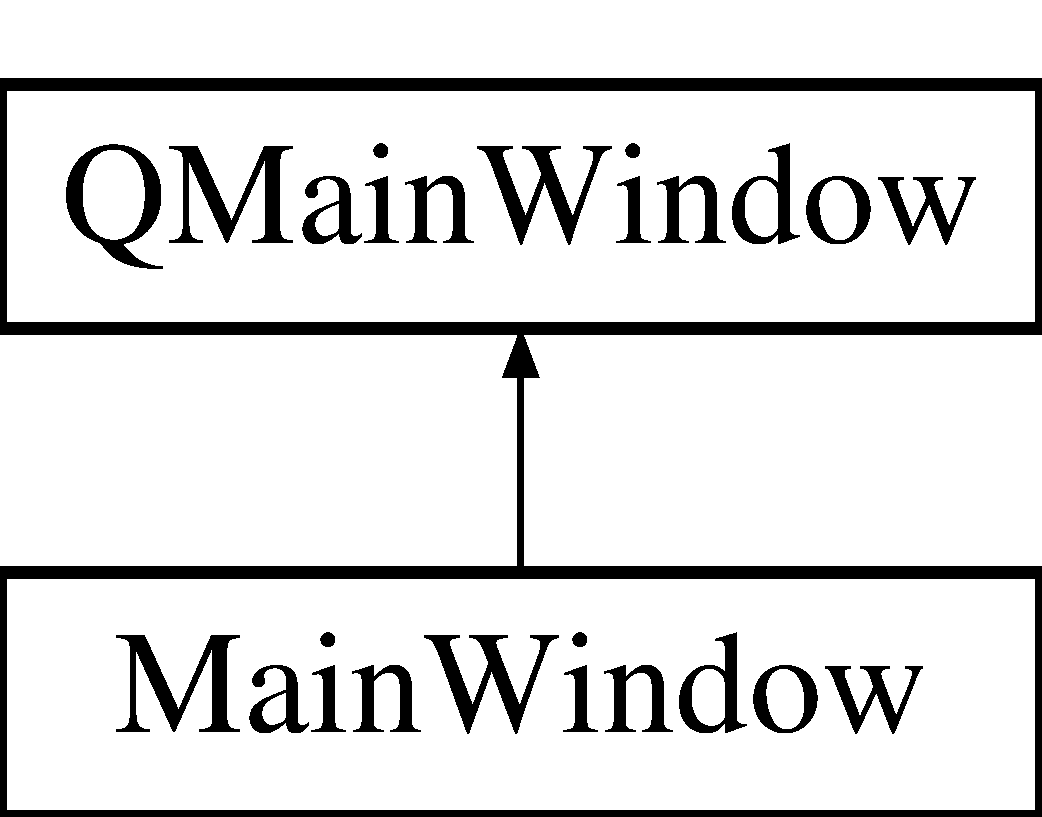
\includegraphics[height=2.000000cm]{class_main_window}
\end{center}
\end{figure}
\subsection*{Public Member Functions}
\begin{DoxyCompactItemize}
\item 
\hyperlink{class_main_window_a996c5a2b6f77944776856f08ec30858d}{Main\+Window} (Q\+Widget $\ast$parent=nullptr)
\item 
\hyperlink{class_main_window_ae98d00a93bc118200eeef9f9bba1dba7}{$\sim$\+Main\+Window} ()
\end{DoxyCompactItemize}
\subsection*{Private Attributes}
\begin{DoxyCompactItemize}
\item 
Ui\+::\+Main\+Window $\ast$ \hyperlink{class_main_window_a35466a70ed47252a0191168126a352a5}{ui}
\end{DoxyCompactItemize}


\subsection{Constructor \& Destructor Documentation}
\mbox{\Hypertarget{class_main_window_a996c5a2b6f77944776856f08ec30858d}\label{class_main_window_a996c5a2b6f77944776856f08ec30858d}} 
\index{Main\+Window@{Main\+Window}!Main\+Window@{Main\+Window}}
\index{Main\+Window@{Main\+Window}!Main\+Window@{Main\+Window}}
\subsubsection{\texorpdfstring{Main\+Window()}{MainWindow()}}
{\footnotesize\ttfamily Main\+Window\+::\+Main\+Window (\begin{DoxyParamCaption}\item[{Q\+Widget $\ast$}]{parent = {\ttfamily nullptr} }\end{DoxyParamCaption})}

\mbox{\Hypertarget{class_main_window_ae98d00a93bc118200eeef9f9bba1dba7}\label{class_main_window_ae98d00a93bc118200eeef9f9bba1dba7}} 
\index{Main\+Window@{Main\+Window}!````~Main\+Window@{$\sim$\+Main\+Window}}
\index{````~Main\+Window@{$\sim$\+Main\+Window}!Main\+Window@{Main\+Window}}
\subsubsection{\texorpdfstring{$\sim$\+Main\+Window()}{~MainWindow()}}
{\footnotesize\ttfamily Main\+Window\+::$\sim$\+Main\+Window (\begin{DoxyParamCaption}{ }\end{DoxyParamCaption})}



\subsection{Member Data Documentation}
\mbox{\Hypertarget{class_main_window_a35466a70ed47252a0191168126a352a5}\label{class_main_window_a35466a70ed47252a0191168126a352a5}} 
\index{Main\+Window@{Main\+Window}!ui@{ui}}
\index{ui@{ui}!Main\+Window@{Main\+Window}}
\subsubsection{\texorpdfstring{ui}{ui}}
{\footnotesize\ttfamily Ui\+::\+Main\+Window$\ast$ Main\+Window\+::ui\hspace{0.3cm}{\ttfamily [private]}}



The documentation for this class was generated from the following files\+:\begin{DoxyCompactItemize}
\item 
/home/kinky\+\_\+tail/se-\/02-\/team-\/24/src/\hyperlink{mainwindow_8h}{mainwindow.\+h}\item 
/home/kinky\+\_\+tail/se-\/02-\/team-\/24/src/\hyperlink{mainwindow_8cpp}{mainwindow.\+cpp}\end{DoxyCompactItemize}

\hypertarget{class_order}{}\section{Order Class Reference}
\label{class_order}\index{Order@{Order}}


{\ttfamily \#include $<$order.\+h$>$}

\subsection*{Public Member Functions}
\begin{DoxyCompactItemize}
\item 
\hyperlink{class_order_a7b6a660b03708ed5b4e1c4a6dc2a664a}{Order} ()
\begin{DoxyCompactList}\small\item\em Default constructor for order. \end{DoxyCompactList}\item 
\hyperlink{class_order_a0c5d4bfa1c8d671665ddd0ecd1cf45d9}{Order} (int n\+\_\+order\+Id, int n\+\_\+g\+ID, int n\+\_\+from\+Player, int n\+\_\+to\+Player, int n\+\_\+ordered\+In\+Week, int n\+\_\+shipped\+Inweek, int n\+\_\+numberof\+Beers)
\begin{DoxyCompactList}\small\item\em Constructor for \hyperlink{class_order}{Order}. \end{DoxyCompactList}\item 
\hyperlink{class_order_a8fb25876ccbd534465f5f96ef9bb2212}{$\sim$\+Order} ()
\begin{DoxyCompactList}\small\item\em distructor for order \end{DoxyCompactList}\item 
void \hyperlink{class_order_a065c7828b1608d906dc9f2f2cc43ee35}{execute\+Order} ()
\begin{DoxyCompactList}\small\item\em Method to execute order. \end{DoxyCompactList}\item 
void \hyperlink{class_order_abb0a14e231e3b3e0d3e59405e3dd9884}{set\+Order\+Id} (int n)
\begin{DoxyCompactList}\small\item\em Setter method for the \hyperlink{class_order}{Order} Id. \end{DoxyCompactList}\item 
void \hyperlink{class_order_a15811f6d8f69a15cc5ca2558328310d6}{set\+G\+Id} (int n)
\begin{DoxyCompactList}\small\item\em Setter method for the \hyperlink{class_game}{Game} Id. \end{DoxyCompactList}\item 
void \hyperlink{class_order_a8a41cdea30959709f9c9dbdadd4f62f0}{set\+From\+Player\+Id} (int n)
\begin{DoxyCompactList}\small\item\em Setter method for the \hyperlink{class_player}{Player} Id of source player of the order. \end{DoxyCompactList}\item 
void \hyperlink{class_order_aea921d19a1a5451eccc92b457c952fba}{set\+To\+Player\+Id} (int n)
\begin{DoxyCompactList}\small\item\em Setter method for the \hyperlink{class_player}{Player} Id of destination player of the order. \end{DoxyCompactList}\item 
void \hyperlink{class_order_aba9a5987294110e6f6dea45feb88c31a}{set\+Ordered\+In\+Week} (int n)
\begin{DoxyCompactList}\small\item\em Setter method for the number of orders in a week. \end{DoxyCompactList}\item 
void \hyperlink{class_order_aac9de21348f84e2556101d52c0ec53af}{set\+Shipped\+In\+Week} (int n)
\begin{DoxyCompactList}\small\item\em Setter method for no of beers shipped in a week. \end{DoxyCompactList}\item 
void \hyperlink{class_order_a5df5676cf7fc84374b5bdb5789aaf2f5}{set\+Number\+Of\+Beers} (int n)
\begin{DoxyCompactList}\small\item\em Setter method for the number of beers in the order. \end{DoxyCompactList}\item 
int \hyperlink{class_order_aa5042da754f07b1876aa63615c5f2983}{get\+Order\+Id} ()
\begin{DoxyCompactList}\small\item\em Getter method for \hyperlink{class_order}{Order} ID. \end{DoxyCompactList}\item 
int \hyperlink{class_order_a89b55df1654ff4cb9db6608fc88c86ed}{get\+G\+Id} ()
\begin{DoxyCompactList}\small\item\em Getter method for \hyperlink{class_game}{Game} ID. \end{DoxyCompactList}\item 
int \hyperlink{class_order_a1d6ae1f551053272307fde77c2cffa58}{get\+From\+Player\+Id} ()
\begin{DoxyCompactList}\small\item\em Getter method for player source ID for the order. \end{DoxyCompactList}\item 
int \hyperlink{class_order_a212e8294656ab9582dbca89de2e1e4c9}{get\+To\+Player\+Id} ()
\begin{DoxyCompactList}\small\item\em Getter method for destinatiion player ID of the order. \end{DoxyCompactList}\item 
int \hyperlink{class_order_aed0ea4435169c95ecc05530df91f225a}{get\+Ordered\+In\+Week} ()
\begin{DoxyCompactList}\small\item\em Getter method for week in which order was ordered. \end{DoxyCompactList}\item 
int \hyperlink{class_order_a7103f60141cf2fefd053aac011dc7613}{get\+Shipped\+In\+Week} ()
\begin{DoxyCompactList}\small\item\em Getter method for number of beers shipped in a week. \end{DoxyCompactList}\item 
int \hyperlink{class_order_a88e86300e6c1b4a21e4ea042b60a7220}{get\+Number\+Of\+Beers} ()
\begin{DoxyCompactList}\small\item\em Getter method for number of beers in that order. \end{DoxyCompactList}\end{DoxyCompactItemize}
\subsection*{Private Attributes}
\begin{DoxyCompactItemize}
\item 
int \hyperlink{class_order_a97409bed7105ee7b4cc7304c18badde0}{orderid}
\begin{DoxyCompactList}\small\item\em Attribute for \hyperlink{class_order}{Order} ID. \end{DoxyCompactList}\item 
int \hyperlink{class_order_a56356acb519b814ab01cfac7864935ff}{gid}
\begin{DoxyCompactList}\small\item\em Attribute for \hyperlink{class_game}{Game} Id. \end{DoxyCompactList}\item 
int \hyperlink{class_order_a6920700bdb4e87fb584c1d95c644b9c2}{from\+Playerid}
\begin{DoxyCompactList}\small\item\em Attribute for describing the source player of order. \end{DoxyCompactList}\item 
int \hyperlink{class_order_a0dd2d933c8d7749a9f1d8d40e4424ab7}{to\+Playerid}
\begin{DoxyCompactList}\small\item\em Attribute for describing the destination player of order. \end{DoxyCompactList}\item 
int \hyperlink{class_order_a5918aa6a6d05f6f4c2f3607094d192d7}{ordered\+In\+Week}
\begin{DoxyCompactList}\small\item\em Attribute for orderes for a week. \end{DoxyCompactList}\item 
int \hyperlink{class_order_ab50c4cb2c20c53d4945fd58dc1e7b395}{shipped\+In\+Week}
\begin{DoxyCompactList}\small\item\em Attribute for orders shipped in a week. \end{DoxyCompactList}\item 
int \hyperlink{class_order_ade9d8347595dcdb4494a5a8d7ebc7cbc}{number\+Of\+Beers}
\begin{DoxyCompactList}\small\item\em Attribute for describing number of beers for the order. \end{DoxyCompactList}\end{DoxyCompactItemize}


\subsection{Constructor \& Destructor Documentation}
\mbox{\Hypertarget{class_order_a7b6a660b03708ed5b4e1c4a6dc2a664a}\label{class_order_a7b6a660b03708ed5b4e1c4a6dc2a664a}} 
\index{Order@{Order}!Order@{Order}}
\index{Order@{Order}!Order@{Order}}
\subsubsection{\texorpdfstring{Order()}{Order()}\hspace{0.1cm}{\footnotesize\ttfamily [1/2]}}
{\footnotesize\ttfamily Order\+::\+Order (\begin{DoxyParamCaption}{ }\end{DoxyParamCaption})}



Default constructor for order. 

\mbox{\Hypertarget{class_order_a0c5d4bfa1c8d671665ddd0ecd1cf45d9}\label{class_order_a0c5d4bfa1c8d671665ddd0ecd1cf45d9}} 
\index{Order@{Order}!Order@{Order}}
\index{Order@{Order}!Order@{Order}}
\subsubsection{\texorpdfstring{Order()}{Order()}\hspace{0.1cm}{\footnotesize\ttfamily [2/2]}}
{\footnotesize\ttfamily Order\+::\+Order (\begin{DoxyParamCaption}\item[{int}]{n\+\_\+order\+Id,  }\item[{int}]{n\+\_\+g\+ID,  }\item[{int}]{n\+\_\+from\+Player,  }\item[{int}]{n\+\_\+to\+Player,  }\item[{int}]{n\+\_\+ordered\+In\+Week,  }\item[{int}]{n\+\_\+shipped\+Inweek,  }\item[{int}]{n\+\_\+numberof\+Beers }\end{DoxyParamCaption})}



Constructor for \hyperlink{class_order}{Order}. 


\begin{DoxyParams}{Parameters}
{\em n\+\_\+order\+Id} & seeting value for order\+Id \\
\hline
{\em n\+\_\+g\+Id} & seeting value for g\+Id \\
\hline
{\em n\+\_\+from\+Id} & seeting value for from\+Id \\
\hline
{\em n\+\_\+to\+Player} & seeting value for o\+Player \\
\hline
{\em n\+\_\+order\+Inweek} & seeting value for order\+Inweek \\
\hline
{\em n\+\_\+shipped\+Inweek} & seeting value for shipped\+Inweek \\
\hline
{\em n\+\_\+numberof\+Beers} & seeting value for numberof\+Beers \\
\hline
\end{DoxyParams}
\mbox{\Hypertarget{class_order_a8fb25876ccbd534465f5f96ef9bb2212}\label{class_order_a8fb25876ccbd534465f5f96ef9bb2212}} 
\index{Order@{Order}!````~Order@{$\sim$\+Order}}
\index{````~Order@{$\sim$\+Order}!Order@{Order}}
\subsubsection{\texorpdfstring{$\sim$\+Order()}{~Order()}}
{\footnotesize\ttfamily Order\+::$\sim$\+Order (\begin{DoxyParamCaption}{ }\end{DoxyParamCaption})}



distructor for order 



\subsection{Member Function Documentation}
\mbox{\Hypertarget{class_order_a065c7828b1608d906dc9f2f2cc43ee35}\label{class_order_a065c7828b1608d906dc9f2f2cc43ee35}} 
\index{Order@{Order}!execute\+Order@{execute\+Order}}
\index{execute\+Order@{execute\+Order}!Order@{Order}}
\subsubsection{\texorpdfstring{execute\+Order()}{executeOrder()}}
{\footnotesize\ttfamily void Order\+::execute\+Order (\begin{DoxyParamCaption}{ }\end{DoxyParamCaption})}



Method to execute order. 

\mbox{\Hypertarget{class_order_a1d6ae1f551053272307fde77c2cffa58}\label{class_order_a1d6ae1f551053272307fde77c2cffa58}} 
\index{Order@{Order}!get\+From\+Player\+Id@{get\+From\+Player\+Id}}
\index{get\+From\+Player\+Id@{get\+From\+Player\+Id}!Order@{Order}}
\subsubsection{\texorpdfstring{get\+From\+Player\+Id()}{getFromPlayerId()}}
{\footnotesize\ttfamily int Order\+::get\+From\+Player\+Id (\begin{DoxyParamCaption}{ }\end{DoxyParamCaption})}



Getter method for player source ID for the order. 

\begin{DoxyReturn}{Returns}
source player ID 
\end{DoxyReturn}
\mbox{\Hypertarget{class_order_a89b55df1654ff4cb9db6608fc88c86ed}\label{class_order_a89b55df1654ff4cb9db6608fc88c86ed}} 
\index{Order@{Order}!get\+G\+Id@{get\+G\+Id}}
\index{get\+G\+Id@{get\+G\+Id}!Order@{Order}}
\subsubsection{\texorpdfstring{get\+G\+Id()}{getGId()}}
{\footnotesize\ttfamily int Order\+::get\+G\+Id (\begin{DoxyParamCaption}{ }\end{DoxyParamCaption})}



Getter method for \hyperlink{class_game}{Game} ID. 

\begin{DoxyReturn}{Returns}
Game\+ID 
\end{DoxyReturn}
\mbox{\Hypertarget{class_order_a88e86300e6c1b4a21e4ea042b60a7220}\label{class_order_a88e86300e6c1b4a21e4ea042b60a7220}} 
\index{Order@{Order}!get\+Number\+Of\+Beers@{get\+Number\+Of\+Beers}}
\index{get\+Number\+Of\+Beers@{get\+Number\+Of\+Beers}!Order@{Order}}
\subsubsection{\texorpdfstring{get\+Number\+Of\+Beers()}{getNumberOfBeers()}}
{\footnotesize\ttfamily int Order\+::get\+Number\+Of\+Beers (\begin{DoxyParamCaption}{ }\end{DoxyParamCaption})}



Getter method for number of beers in that order. 

\begin{DoxyReturn}{Returns}
number of beers in that order 
\end{DoxyReturn}
\mbox{\Hypertarget{class_order_aed0ea4435169c95ecc05530df91f225a}\label{class_order_aed0ea4435169c95ecc05530df91f225a}} 
\index{Order@{Order}!get\+Ordered\+In\+Week@{get\+Ordered\+In\+Week}}
\index{get\+Ordered\+In\+Week@{get\+Ordered\+In\+Week}!Order@{Order}}
\subsubsection{\texorpdfstring{get\+Ordered\+In\+Week()}{getOrderedInWeek()}}
{\footnotesize\ttfamily int Order\+::get\+Ordered\+In\+Week (\begin{DoxyParamCaption}{ }\end{DoxyParamCaption})}



Getter method for week in which order was ordered. 

\begin{DoxyReturn}{Returns}
week no of orderd week 
\end{DoxyReturn}
\mbox{\Hypertarget{class_order_aa5042da754f07b1876aa63615c5f2983}\label{class_order_aa5042da754f07b1876aa63615c5f2983}} 
\index{Order@{Order}!get\+Order\+Id@{get\+Order\+Id}}
\index{get\+Order\+Id@{get\+Order\+Id}!Order@{Order}}
\subsubsection{\texorpdfstring{get\+Order\+Id()}{getOrderId()}}
{\footnotesize\ttfamily int Order\+::get\+Order\+Id (\begin{DoxyParamCaption}{ }\end{DoxyParamCaption})}



Getter method for \hyperlink{class_order}{Order} ID. 

\begin{DoxyReturn}{Returns}
\hyperlink{class_order}{Order} ID 
\end{DoxyReturn}
\mbox{\Hypertarget{class_order_a7103f60141cf2fefd053aac011dc7613}\label{class_order_a7103f60141cf2fefd053aac011dc7613}} 
\index{Order@{Order}!get\+Shipped\+In\+Week@{get\+Shipped\+In\+Week}}
\index{get\+Shipped\+In\+Week@{get\+Shipped\+In\+Week}!Order@{Order}}
\subsubsection{\texorpdfstring{get\+Shipped\+In\+Week()}{getShippedInWeek()}}
{\footnotesize\ttfamily int Order\+::get\+Shipped\+In\+Week (\begin{DoxyParamCaption}{ }\end{DoxyParamCaption})}



Getter method for number of beers shipped in a week. 

\begin{DoxyReturn}{Returns}
beers shipped in the week 
\end{DoxyReturn}
\mbox{\Hypertarget{class_order_a212e8294656ab9582dbca89de2e1e4c9}\label{class_order_a212e8294656ab9582dbca89de2e1e4c9}} 
\index{Order@{Order}!get\+To\+Player\+Id@{get\+To\+Player\+Id}}
\index{get\+To\+Player\+Id@{get\+To\+Player\+Id}!Order@{Order}}
\subsubsection{\texorpdfstring{get\+To\+Player\+Id()}{getToPlayerId()}}
{\footnotesize\ttfamily int Order\+::get\+To\+Player\+Id (\begin{DoxyParamCaption}{ }\end{DoxyParamCaption})}



Getter method for destinatiion player ID of the order. 

\begin{DoxyReturn}{Returns}
destination player ID 
\end{DoxyReturn}
\mbox{\Hypertarget{class_order_a8a41cdea30959709f9c9dbdadd4f62f0}\label{class_order_a8a41cdea30959709f9c9dbdadd4f62f0}} 
\index{Order@{Order}!set\+From\+Player\+Id@{set\+From\+Player\+Id}}
\index{set\+From\+Player\+Id@{set\+From\+Player\+Id}!Order@{Order}}
\subsubsection{\texorpdfstring{set\+From\+Player\+Id()}{setFromPlayerId()}}
{\footnotesize\ttfamily void Order\+::set\+From\+Player\+Id (\begin{DoxyParamCaption}\item[{int}]{n }\end{DoxyParamCaption})}



Setter method for the \hyperlink{class_player}{Player} Id of source player of the order. 


\begin{DoxyParams}{Parameters}
{\em n} & seeting value for player Id \\
\hline
\end{DoxyParams}
\mbox{\Hypertarget{class_order_a15811f6d8f69a15cc5ca2558328310d6}\label{class_order_a15811f6d8f69a15cc5ca2558328310d6}} 
\index{Order@{Order}!set\+G\+Id@{set\+G\+Id}}
\index{set\+G\+Id@{set\+G\+Id}!Order@{Order}}
\subsubsection{\texorpdfstring{set\+G\+Id()}{setGId()}}
{\footnotesize\ttfamily void Order\+::set\+G\+Id (\begin{DoxyParamCaption}\item[{int}]{n }\end{DoxyParamCaption})}



Setter method for the \hyperlink{class_game}{Game} Id. 


\begin{DoxyParams}{Parameters}
{\em n} & seeting value for \hyperlink{class_game}{Game} Id \\
\hline
\end{DoxyParams}
\mbox{\Hypertarget{class_order_a5df5676cf7fc84374b5bdb5789aaf2f5}\label{class_order_a5df5676cf7fc84374b5bdb5789aaf2f5}} 
\index{Order@{Order}!set\+Number\+Of\+Beers@{set\+Number\+Of\+Beers}}
\index{set\+Number\+Of\+Beers@{set\+Number\+Of\+Beers}!Order@{Order}}
\subsubsection{\texorpdfstring{set\+Number\+Of\+Beers()}{setNumberOfBeers()}}
{\footnotesize\ttfamily void Order\+::set\+Number\+Of\+Beers (\begin{DoxyParamCaption}\item[{int}]{n }\end{DoxyParamCaption})}



Setter method for the number of beers in the order. 


\begin{DoxyParams}{Parameters}
{\em n} & seeting value for Number of beers \\
\hline
\end{DoxyParams}
\mbox{\Hypertarget{class_order_aba9a5987294110e6f6dea45feb88c31a}\label{class_order_aba9a5987294110e6f6dea45feb88c31a}} 
\index{Order@{Order}!set\+Ordered\+In\+Week@{set\+Ordered\+In\+Week}}
\index{set\+Ordered\+In\+Week@{set\+Ordered\+In\+Week}!Order@{Order}}
\subsubsection{\texorpdfstring{set\+Ordered\+In\+Week()}{setOrderedInWeek()}}
{\footnotesize\ttfamily void Order\+::set\+Ordered\+In\+Week (\begin{DoxyParamCaption}\item[{int}]{n }\end{DoxyParamCaption})}



Setter method for the number of orders in a week. 


\begin{DoxyParams}{Parameters}
{\em n} & seeting value for Ordered\+In\+Week \\
\hline
\end{DoxyParams}
\mbox{\Hypertarget{class_order_abb0a14e231e3b3e0d3e59405e3dd9884}\label{class_order_abb0a14e231e3b3e0d3e59405e3dd9884}} 
\index{Order@{Order}!set\+Order\+Id@{set\+Order\+Id}}
\index{set\+Order\+Id@{set\+Order\+Id}!Order@{Order}}
\subsubsection{\texorpdfstring{set\+Order\+Id()}{setOrderId()}}
{\footnotesize\ttfamily void Order\+::set\+Order\+Id (\begin{DoxyParamCaption}\item[{int}]{n }\end{DoxyParamCaption})}



Setter method for the \hyperlink{class_order}{Order} Id. 


\begin{DoxyParams}{Parameters}
{\em n} & seeting value for \hyperlink{class_order}{Order} Id \\
\hline
\end{DoxyParams}
\mbox{\Hypertarget{class_order_aac9de21348f84e2556101d52c0ec53af}\label{class_order_aac9de21348f84e2556101d52c0ec53af}} 
\index{Order@{Order}!set\+Shipped\+In\+Week@{set\+Shipped\+In\+Week}}
\index{set\+Shipped\+In\+Week@{set\+Shipped\+In\+Week}!Order@{Order}}
\subsubsection{\texorpdfstring{set\+Shipped\+In\+Week()}{setShippedInWeek()}}
{\footnotesize\ttfamily void Order\+::set\+Shipped\+In\+Week (\begin{DoxyParamCaption}\item[{int}]{n }\end{DoxyParamCaption})}



Setter method for no of beers shipped in a week. 


\begin{DoxyParams}{Parameters}
{\em n} & seeting value for Shipped in week \\
\hline
\end{DoxyParams}
\mbox{\Hypertarget{class_order_aea921d19a1a5451eccc92b457c952fba}\label{class_order_aea921d19a1a5451eccc92b457c952fba}} 
\index{Order@{Order}!set\+To\+Player\+Id@{set\+To\+Player\+Id}}
\index{set\+To\+Player\+Id@{set\+To\+Player\+Id}!Order@{Order}}
\subsubsection{\texorpdfstring{set\+To\+Player\+Id()}{setToPlayerId()}}
{\footnotesize\ttfamily void Order\+::set\+To\+Player\+Id (\begin{DoxyParamCaption}\item[{int}]{n }\end{DoxyParamCaption})}



Setter method for the \hyperlink{class_player}{Player} Id of destination player of the order. 


\begin{DoxyParams}{Parameters}
{\em n} & seeting value for player Id \\
\hline
\end{DoxyParams}


\subsection{Member Data Documentation}
\mbox{\Hypertarget{class_order_a6920700bdb4e87fb584c1d95c644b9c2}\label{class_order_a6920700bdb4e87fb584c1d95c644b9c2}} 
\index{Order@{Order}!from\+Playerid@{from\+Playerid}}
\index{from\+Playerid@{from\+Playerid}!Order@{Order}}
\subsubsection{\texorpdfstring{from\+Playerid}{fromPlayerid}}
{\footnotesize\ttfamily int Order\+::from\+Playerid\hspace{0.3cm}{\ttfamily [private]}}



Attribute for describing the source player of order. 

\mbox{\Hypertarget{class_order_a56356acb519b814ab01cfac7864935ff}\label{class_order_a56356acb519b814ab01cfac7864935ff}} 
\index{Order@{Order}!gid@{gid}}
\index{gid@{gid}!Order@{Order}}
\subsubsection{\texorpdfstring{gid}{gid}}
{\footnotesize\ttfamily int Order\+::gid\hspace{0.3cm}{\ttfamily [private]}}



Attribute for \hyperlink{class_game}{Game} Id. 

\mbox{\Hypertarget{class_order_ade9d8347595dcdb4494a5a8d7ebc7cbc}\label{class_order_ade9d8347595dcdb4494a5a8d7ebc7cbc}} 
\index{Order@{Order}!number\+Of\+Beers@{number\+Of\+Beers}}
\index{number\+Of\+Beers@{number\+Of\+Beers}!Order@{Order}}
\subsubsection{\texorpdfstring{number\+Of\+Beers}{numberOfBeers}}
{\footnotesize\ttfamily int Order\+::number\+Of\+Beers\hspace{0.3cm}{\ttfamily [private]}}



Attribute for describing number of beers for the order. 

\mbox{\Hypertarget{class_order_a5918aa6a6d05f6f4c2f3607094d192d7}\label{class_order_a5918aa6a6d05f6f4c2f3607094d192d7}} 
\index{Order@{Order}!ordered\+In\+Week@{ordered\+In\+Week}}
\index{ordered\+In\+Week@{ordered\+In\+Week}!Order@{Order}}
\subsubsection{\texorpdfstring{ordered\+In\+Week}{orderedInWeek}}
{\footnotesize\ttfamily int Order\+::ordered\+In\+Week\hspace{0.3cm}{\ttfamily [private]}}



Attribute for orderes for a week. 

\mbox{\Hypertarget{class_order_a97409bed7105ee7b4cc7304c18badde0}\label{class_order_a97409bed7105ee7b4cc7304c18badde0}} 
\index{Order@{Order}!orderid@{orderid}}
\index{orderid@{orderid}!Order@{Order}}
\subsubsection{\texorpdfstring{orderid}{orderid}}
{\footnotesize\ttfamily int Order\+::orderid\hspace{0.3cm}{\ttfamily [private]}}



Attribute for \hyperlink{class_order}{Order} ID. 

\mbox{\Hypertarget{class_order_ab50c4cb2c20c53d4945fd58dc1e7b395}\label{class_order_ab50c4cb2c20c53d4945fd58dc1e7b395}} 
\index{Order@{Order}!shipped\+In\+Week@{shipped\+In\+Week}}
\index{shipped\+In\+Week@{shipped\+In\+Week}!Order@{Order}}
\subsubsection{\texorpdfstring{shipped\+In\+Week}{shippedInWeek}}
{\footnotesize\ttfamily int Order\+::shipped\+In\+Week\hspace{0.3cm}{\ttfamily [private]}}



Attribute for orders shipped in a week. 

\mbox{\Hypertarget{class_order_a0dd2d933c8d7749a9f1d8d40e4424ab7}\label{class_order_a0dd2d933c8d7749a9f1d8d40e4424ab7}} 
\index{Order@{Order}!to\+Playerid@{to\+Playerid}}
\index{to\+Playerid@{to\+Playerid}!Order@{Order}}
\subsubsection{\texorpdfstring{to\+Playerid}{toPlayerid}}
{\footnotesize\ttfamily int Order\+::to\+Playerid\hspace{0.3cm}{\ttfamily [private]}}



Attribute for describing the destination player of order. 



The documentation for this class was generated from the following files\+:\begin{DoxyCompactItemize}
\item 
/home/kinky\+\_\+tail/se-\/02-\/team-\/24/src/\hyperlink{order_8h}{order.\+h}\item 
/home/kinky\+\_\+tail/se-\/02-\/team-\/24/src/\hyperlink{order_8cpp}{order.\+cpp}\end{DoxyCompactItemize}

\hypertarget{class_player}{}\section{Player Class Reference}
\label{class_player}\index{Player@{Player}}


{\ttfamily \#include $<$player.\+h$>$}

Inheritance diagram for Player\+:\begin{figure}[H]
\begin{center}
\leavevmode
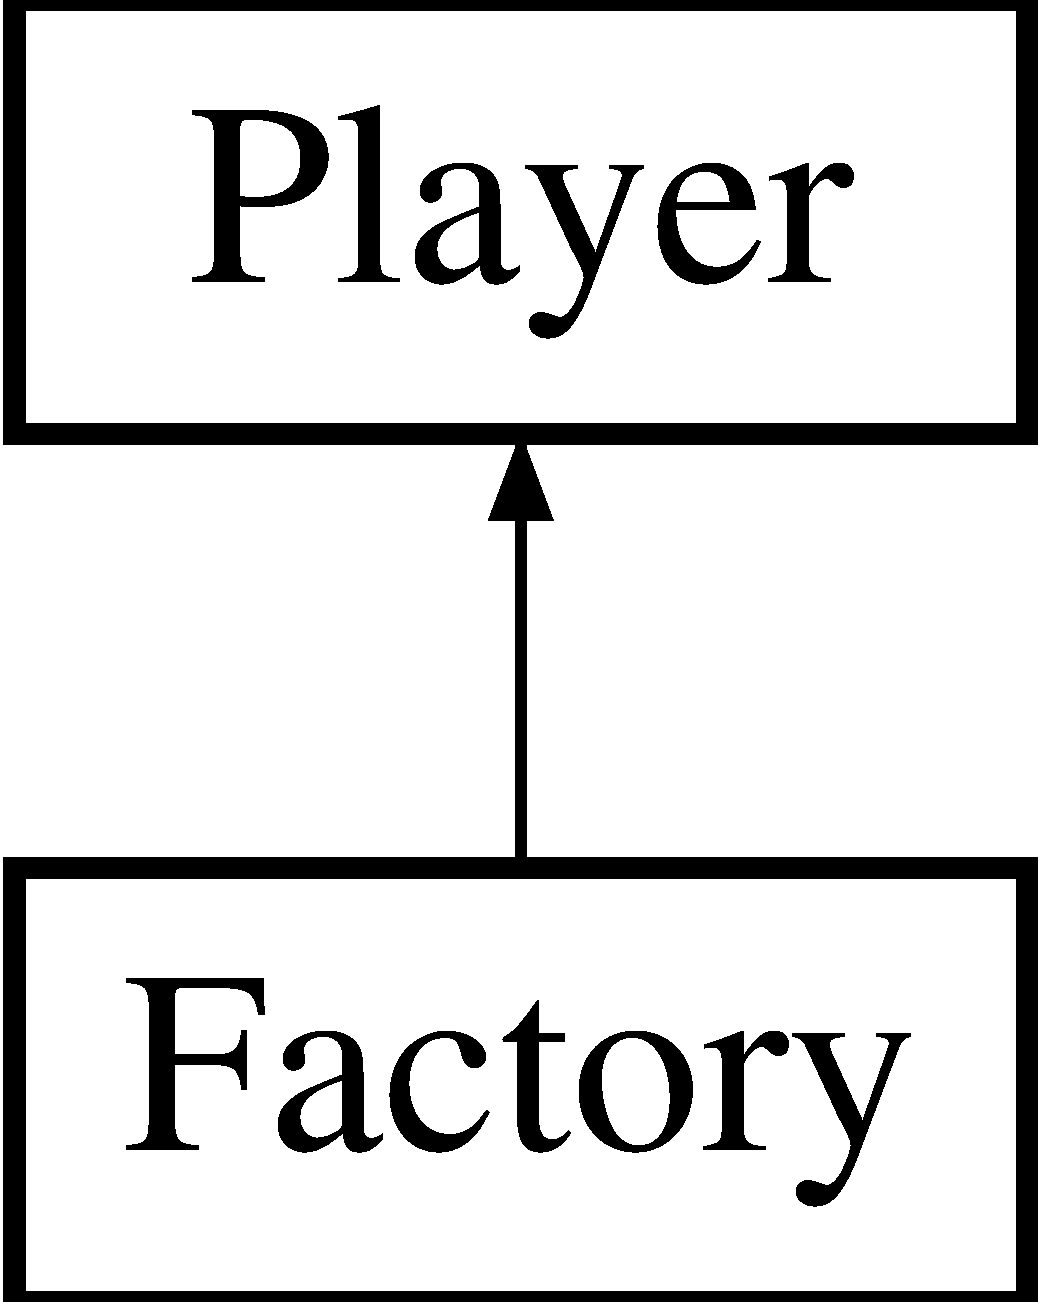
\includegraphics[height=2.000000cm]{class_player}
\end{center}
\end{figure}
\subsection*{Public Member Functions}
\begin{DoxyCompactItemize}
\item 
\hyperlink{class_player_affe0cc3cb714f6deb4e62f0c0d3f1fd8}{Player} ()
\begin{DoxyCompactList}\small\item\em Constructor for game class, sets the default values for game class. \end{DoxyCompactList}\item 
\hyperlink{class_player_a8fd722300bd72d1d043e789e7ed2a39b}{Player} (int n\+\_\+role)
\begin{DoxyCompactList}\small\item\em Constructor for game class, sets the default values for game class. \end{DoxyCompactList}\item 
\hyperlink{class_player_a749d2c00e1fe0f5c2746f7505a58c062}{$\sim$\+Player} ()
\begin{DoxyCompactList}\small\item\em distructor for game class \end{DoxyCompactList}\item 
void \hyperlink{class_player_a473d9c248207e213abc5575859a51c1b}{order} (int number\+Of\+Beers, \hyperlink{class_player}{Player} from)
\begin{DoxyCompactList}\small\item\em Method to order a shipment from a player. \end{DoxyCompactList}\item 
void \hyperlink{class_player_a68db574596d1ca040f454d34310149ee}{ship} (int number\+Of\+Beers, \hyperlink{class_player}{Player} to)
\begin{DoxyCompactList}\small\item\em Method to ship a shipment to the player. \end{DoxyCompactList}\item 
int \hyperlink{class_player_ae2197d1061a24fa444129b5ea85996d5}{decrease\+Inventory} (int number\+Of\+Beers)
\begin{DoxyCompactList}\small\item\em Method to decrease inventory. \end{DoxyCompactList}\item 
int \hyperlink{class_player_af67e6ee0de38f3e9635d35849f103449}{increase\+Inventory} (int number\+Of\+Beers)
\begin{DoxyCompactList}\small\item\em Method to increase inventory. \end{DoxyCompactList}\item 
void \hyperlink{class_player_afd48e4062a9411e1f66cf23809b8c43f}{receive\+Shipment} (int order\+ID)
\begin{DoxyCompactList}\small\item\em Method to receive Shipment. \end{DoxyCompactList}\item 
void \hyperlink{class_player_a534f0e79b1e7a6310f3d02e04b95b4b4}{set\+P\+Id} (int n\+\_\+\+P\+Id)
\begin{DoxyCompactList}\small\item\em Setter method for the \hyperlink{class_player}{Player} Id. \end{DoxyCompactList}\item 
void \hyperlink{class_player_a5def6f94584d296aaba2d620697a8922}{set\+Role} (int n\+\_\+role)
\begin{DoxyCompactList}\small\item\em Setter method for the \hyperlink{class_player}{Player} role. \end{DoxyCompactList}\item 
void \hyperlink{class_player_a279e316b279fcf5e78f395bea0f417f0}{set\+Inventory} (int n\+\_\+inventory)
\begin{DoxyCompactList}\small\item\em Setter method for the \hyperlink{class_player}{Player} Inventory. \end{DoxyCompactList}\item 
void \hyperlink{class_player_a55cf59cc96744fee031167b7736e5d35}{set\+Backorder} (int n\+\_\+backorder)
\begin{DoxyCompactList}\small\item\em Setter method for the \hyperlink{class_player}{Player}\textquotesingle{}s backorder. \end{DoxyCompactList}\item 
void \hyperlink{class_player_adae26798d67d12ad53bd3d9ba2e8b0fc}{set\+Cost} (int n\+\_\+cost)
\begin{DoxyCompactList}\small\item\em Setter method for the \hyperlink{class_player}{Player}\textquotesingle{}s cost. \end{DoxyCompactList}\item 
void \hyperlink{class_player_aba795131e99318dfc9d4fef7de189aac}{set\+Demand} (int n\+\_\+demand)
\begin{DoxyCompactList}\small\item\em Setter method for the Players\textquotesingle{}s demand. \end{DoxyCompactList}\item 
void \hyperlink{class_player_ab197bac4da8cbf646c6ffa36a16ad0b0}{set\+Order\+Placed} (int n\+\_\+order)
\begin{DoxyCompactList}\small\item\em Setter method for the \hyperlink{class_player}{Player}\textquotesingle{}s order to be placed. \end{DoxyCompactList}\item 
int \hyperlink{class_player_ad815840dfa1c1261900774b5ffd886e3}{get\+P\+Id} ()
\begin{DoxyCompactList}\small\item\em Getter method for \hyperlink{class_player}{Player} Id. \end{DoxyCompactList}\item 
int \hyperlink{class_player_a6baeff2a6218449299cb334c01f1dc28}{get\+Role} ()
\begin{DoxyCompactList}\small\item\em Getter method for \hyperlink{class_player}{Player}\textquotesingle{}s role in the game. \end{DoxyCompactList}\item 
int \hyperlink{class_player_ae21d65a545c20c70ac7a53389b223ce6}{get\+Inventory} ()
\begin{DoxyCompactList}\small\item\em Getter method for player\textquotesingle{}s inventory. \end{DoxyCompactList}\item 
int \hyperlink{class_player_a8080e44c26141d956babb824d2a7ae7c}{get\+Backorder} ()
\begin{DoxyCompactList}\small\item\em Getter method for backorder cost. \end{DoxyCompactList}\item 
int \hyperlink{class_player_a3a1e9666f1da8750452296310ed95e1f}{get\+Cost} ()
\begin{DoxyCompactList}\small\item\em Getter method for player\textquotesingle{}s cost. \end{DoxyCompactList}\item 
int \hyperlink{class_player_a8bfca991628b682ff9cae6d05ee9131c}{get\+Demand} ()
\begin{DoxyCompactList}\small\item\em Getter method for demand of player. \end{DoxyCompactList}\item 
int \hyperlink{class_player_af838b44639ee94d4185917d5d2259ce2}{get\+Order\+Placed} ()
\begin{DoxyCompactList}\small\item\em Getter method for order to be placed. \end{DoxyCompactList}\end{DoxyCompactItemize}
\subsection*{Private Attributes}
\begin{DoxyCompactItemize}
\item 
int \hyperlink{class_player_aa450b5b5cdda7cae086fb28a78d1fb8c}{p\+Id}
\begin{DoxyCompactList}\small\item\em Attribute for \hyperlink{class_player}{Player} Id. \end{DoxyCompactList}\item 
int \hyperlink{class_player_a3544f9c49c57c160a3edae988d1fae42}{role}
\begin{DoxyCompactList}\small\item\em Attribute for role of player in game. \end{DoxyCompactList}\item 
int \hyperlink{class_player_a68e4cf30506015d9291ffc4c1c5b1078}{inventory}
\begin{DoxyCompactList}\small\item\em Attribute for current inventory of the player. \end{DoxyCompactList}\item 
double \hyperlink{class_player_a691751190c6389e1aef1b5b949cb11b7}{backorder}
\begin{DoxyCompactList}\small\item\em Attribute for current backorder of the player. \end{DoxyCompactList}\item 
double \hyperlink{class_player_a7477b3893f2805a36042e96b4aeb2151}{cost}
\begin{DoxyCompactList}\small\item\em Attribute for current cost of player in the game. \end{DoxyCompactList}\item 
int \hyperlink{class_player_aec98bfa93606a2b7cf4978c7d500917b}{demand}
\begin{DoxyCompactList}\small\item\em Attribute for current demand of player in game. \end{DoxyCompactList}\item 
int \hyperlink{class_player_a5ce498c11486dc2994a9ab7f3ba24260}{order\+Placed}
\begin{DoxyCompactList}\small\item\em Attribute for order placed by the player. \end{DoxyCompactList}\end{DoxyCompactItemize}


\subsection{Constructor \& Destructor Documentation}
\mbox{\Hypertarget{class_player_affe0cc3cb714f6deb4e62f0c0d3f1fd8}\label{class_player_affe0cc3cb714f6deb4e62f0c0d3f1fd8}} 
\index{Player@{Player}!Player@{Player}}
\index{Player@{Player}!Player@{Player}}
\subsubsection{\texorpdfstring{Player()}{Player()}\hspace{0.1cm}{\footnotesize\ttfamily [1/2]}}
{\footnotesize\ttfamily Player\+::\+Player (\begin{DoxyParamCaption}{ }\end{DoxyParamCaption})}



Constructor for game class, sets the default values for game class. 

\mbox{\Hypertarget{class_player_a8fd722300bd72d1d043e789e7ed2a39b}\label{class_player_a8fd722300bd72d1d043e789e7ed2a39b}} 
\index{Player@{Player}!Player@{Player}}
\index{Player@{Player}!Player@{Player}}
\subsubsection{\texorpdfstring{Player()}{Player()}\hspace{0.1cm}{\footnotesize\ttfamily [2/2]}}
{\footnotesize\ttfamily Player\+::\+Player (\begin{DoxyParamCaption}\item[{int}]{n\+\_\+role }\end{DoxyParamCaption})}



Constructor for game class, sets the default values for game class. 


\begin{DoxyParams}{Parameters}
{\em n\+\_\+role} & seeting value for player role in the game \\
\hline
\end{DoxyParams}
\mbox{\Hypertarget{class_player_a749d2c00e1fe0f5c2746f7505a58c062}\label{class_player_a749d2c00e1fe0f5c2746f7505a58c062}} 
\index{Player@{Player}!````~Player@{$\sim$\+Player}}
\index{````~Player@{$\sim$\+Player}!Player@{Player}}
\subsubsection{\texorpdfstring{$\sim$\+Player()}{~Player()}}
{\footnotesize\ttfamily Player\+::$\sim$\+Player (\begin{DoxyParamCaption}{ }\end{DoxyParamCaption})}



distructor for game class 



\subsection{Member Function Documentation}
\mbox{\Hypertarget{class_player_ae2197d1061a24fa444129b5ea85996d5}\label{class_player_ae2197d1061a24fa444129b5ea85996d5}} 
\index{Player@{Player}!decrease\+Inventory@{decrease\+Inventory}}
\index{decrease\+Inventory@{decrease\+Inventory}!Player@{Player}}
\subsubsection{\texorpdfstring{decrease\+Inventory()}{decreaseInventory()}}
{\footnotesize\ttfamily int Player\+::decrease\+Inventory (\begin{DoxyParamCaption}\item[{int}]{number\+Of\+Beers }\end{DoxyParamCaption})}



Method to decrease inventory. 


\begin{DoxyParams}{Parameters}
{\em number\+Of\+Beers} & is number of beers to be decreased in the inventory \\
\hline
\end{DoxyParams}
\mbox{\Hypertarget{class_player_a8080e44c26141d956babb824d2a7ae7c}\label{class_player_a8080e44c26141d956babb824d2a7ae7c}} 
\index{Player@{Player}!get\+Backorder@{get\+Backorder}}
\index{get\+Backorder@{get\+Backorder}!Player@{Player}}
\subsubsection{\texorpdfstring{get\+Backorder()}{getBackorder()}}
{\footnotesize\ttfamily int Player\+::get\+Backorder (\begin{DoxyParamCaption}{ }\end{DoxyParamCaption})}



Getter method for backorder cost. 

\begin{DoxyReturn}{Returns}
backorder cost 
\end{DoxyReturn}
\mbox{\Hypertarget{class_player_a3a1e9666f1da8750452296310ed95e1f}\label{class_player_a3a1e9666f1da8750452296310ed95e1f}} 
\index{Player@{Player}!get\+Cost@{get\+Cost}}
\index{get\+Cost@{get\+Cost}!Player@{Player}}
\subsubsection{\texorpdfstring{get\+Cost()}{getCost()}}
{\footnotesize\ttfamily int Player\+::get\+Cost (\begin{DoxyParamCaption}{ }\end{DoxyParamCaption})}



Getter method for player\textquotesingle{}s cost. 

\begin{DoxyReturn}{Returns}
cost 
\end{DoxyReturn}
\mbox{\Hypertarget{class_player_a8bfca991628b682ff9cae6d05ee9131c}\label{class_player_a8bfca991628b682ff9cae6d05ee9131c}} 
\index{Player@{Player}!get\+Demand@{get\+Demand}}
\index{get\+Demand@{get\+Demand}!Player@{Player}}
\subsubsection{\texorpdfstring{get\+Demand()}{getDemand()}}
{\footnotesize\ttfamily int Player\+::get\+Demand (\begin{DoxyParamCaption}{ }\end{DoxyParamCaption})}



Getter method for demand of player. 

\begin{DoxyReturn}{Returns}
player id 
\end{DoxyReturn}
\mbox{\Hypertarget{class_player_ae21d65a545c20c70ac7a53389b223ce6}\label{class_player_ae21d65a545c20c70ac7a53389b223ce6}} 
\index{Player@{Player}!get\+Inventory@{get\+Inventory}}
\index{get\+Inventory@{get\+Inventory}!Player@{Player}}
\subsubsection{\texorpdfstring{get\+Inventory()}{getInventory()}}
{\footnotesize\ttfamily int Player\+::get\+Inventory (\begin{DoxyParamCaption}{ }\end{DoxyParamCaption})}



Getter method for player\textquotesingle{}s inventory. 

\begin{DoxyReturn}{Returns}
player\textquotesingle{}s inventory 
\end{DoxyReturn}
\mbox{\Hypertarget{class_player_af838b44639ee94d4185917d5d2259ce2}\label{class_player_af838b44639ee94d4185917d5d2259ce2}} 
\index{Player@{Player}!get\+Order\+Placed@{get\+Order\+Placed}}
\index{get\+Order\+Placed@{get\+Order\+Placed}!Player@{Player}}
\subsubsection{\texorpdfstring{get\+Order\+Placed()}{getOrderPlaced()}}
{\footnotesize\ttfamily int Player\+::get\+Order\+Placed (\begin{DoxyParamCaption}{ }\end{DoxyParamCaption})}



Getter method for order to be placed. 

\begin{DoxyReturn}{Returns}
order placed 
\end{DoxyReturn}
\mbox{\Hypertarget{class_player_ad815840dfa1c1261900774b5ffd886e3}\label{class_player_ad815840dfa1c1261900774b5ffd886e3}} 
\index{Player@{Player}!get\+P\+Id@{get\+P\+Id}}
\index{get\+P\+Id@{get\+P\+Id}!Player@{Player}}
\subsubsection{\texorpdfstring{get\+P\+Id()}{getPId()}}
{\footnotesize\ttfamily int Player\+::get\+P\+Id (\begin{DoxyParamCaption}{ }\end{DoxyParamCaption})}



Getter method for \hyperlink{class_player}{Player} Id. 

\begin{DoxyReturn}{Returns}
\hyperlink{class_instructor}{Instructor} Id 
\end{DoxyReturn}
\mbox{\Hypertarget{class_player_a6baeff2a6218449299cb334c01f1dc28}\label{class_player_a6baeff2a6218449299cb334c01f1dc28}} 
\index{Player@{Player}!get\+Role@{get\+Role}}
\index{get\+Role@{get\+Role}!Player@{Player}}
\subsubsection{\texorpdfstring{get\+Role()}{getRole()}}
{\footnotesize\ttfamily int Player\+::get\+Role (\begin{DoxyParamCaption}{ }\end{DoxyParamCaption})}



Getter method for \hyperlink{class_player}{Player}\textquotesingle{}s role in the game. 

\begin{DoxyReturn}{Returns}
role 
\end{DoxyReturn}
\mbox{\Hypertarget{class_player_af67e6ee0de38f3e9635d35849f103449}\label{class_player_af67e6ee0de38f3e9635d35849f103449}} 
\index{Player@{Player}!increase\+Inventory@{increase\+Inventory}}
\index{increase\+Inventory@{increase\+Inventory}!Player@{Player}}
\subsubsection{\texorpdfstring{increase\+Inventory()}{increaseInventory()}}
{\footnotesize\ttfamily int Player\+::increase\+Inventory (\begin{DoxyParamCaption}\item[{int}]{number\+Of\+Beers }\end{DoxyParamCaption})}



Method to increase inventory. 


\begin{DoxyParams}{Parameters}
{\em number\+Of\+Beers} & is number of beers to be increased in the inventory \\
\hline
\end{DoxyParams}
\mbox{\Hypertarget{class_player_a473d9c248207e213abc5575859a51c1b}\label{class_player_a473d9c248207e213abc5575859a51c1b}} 
\index{Player@{Player}!order@{order}}
\index{order@{order}!Player@{Player}}
\subsubsection{\texorpdfstring{order()}{order()}}
{\footnotesize\ttfamily void Player\+::order (\begin{DoxyParamCaption}\item[{int}]{number\+Of\+Beers,  }\item[{\hyperlink{class_player}{Player}}]{from }\end{DoxyParamCaption})}



Method to order a shipment from a player. 


\begin{DoxyParams}{Parameters}
{\em number\+Of\+Beers} & is number of beers to be ordered \\
\hline
{\em From} & is the player from where the order is ordered \\
\hline
\end{DoxyParams}
\mbox{\Hypertarget{class_player_afd48e4062a9411e1f66cf23809b8c43f}\label{class_player_afd48e4062a9411e1f66cf23809b8c43f}} 
\index{Player@{Player}!receive\+Shipment@{receive\+Shipment}}
\index{receive\+Shipment@{receive\+Shipment}!Player@{Player}}
\subsubsection{\texorpdfstring{receive\+Shipment()}{receiveShipment()}}
{\footnotesize\ttfamily void Player\+::receive\+Shipment (\begin{DoxyParamCaption}\item[{int}]{order\+ID }\end{DoxyParamCaption})}



Method to receive Shipment. 


\begin{DoxyParams}{Parameters}
{\em Order\+ID} & is id of order to be received \\
\hline
\end{DoxyParams}
\mbox{\Hypertarget{class_player_a55cf59cc96744fee031167b7736e5d35}\label{class_player_a55cf59cc96744fee031167b7736e5d35}} 
\index{Player@{Player}!set\+Backorder@{set\+Backorder}}
\index{set\+Backorder@{set\+Backorder}!Player@{Player}}
\subsubsection{\texorpdfstring{set\+Backorder()}{setBackorder()}}
{\footnotesize\ttfamily void Player\+::set\+Backorder (\begin{DoxyParamCaption}\item[{int}]{n\+\_\+backorder }\end{DoxyParamCaption})}



Setter method for the \hyperlink{class_player}{Player}\textquotesingle{}s backorder. 


\begin{DoxyParams}{Parameters}
{\em n\+\_\+backorder} & seeting value for player\textquotesingle{}s backorder \\
\hline
\end{DoxyParams}
\mbox{\Hypertarget{class_player_adae26798d67d12ad53bd3d9ba2e8b0fc}\label{class_player_adae26798d67d12ad53bd3d9ba2e8b0fc}} 
\index{Player@{Player}!set\+Cost@{set\+Cost}}
\index{set\+Cost@{set\+Cost}!Player@{Player}}
\subsubsection{\texorpdfstring{set\+Cost()}{setCost()}}
{\footnotesize\ttfamily void Player\+::set\+Cost (\begin{DoxyParamCaption}\item[{int}]{n\+\_\+cost }\end{DoxyParamCaption})}



Setter method for the \hyperlink{class_player}{Player}\textquotesingle{}s cost. 


\begin{DoxyParams}{Parameters}
{\em n\+\_\+cost} & seeting value for player\textquotesingle{}s cost \\
\hline
\end{DoxyParams}
\mbox{\Hypertarget{class_player_aba795131e99318dfc9d4fef7de189aac}\label{class_player_aba795131e99318dfc9d4fef7de189aac}} 
\index{Player@{Player}!set\+Demand@{set\+Demand}}
\index{set\+Demand@{set\+Demand}!Player@{Player}}
\subsubsection{\texorpdfstring{set\+Demand()}{setDemand()}}
{\footnotesize\ttfamily void Player\+::set\+Demand (\begin{DoxyParamCaption}\item[{int}]{n\+\_\+demand }\end{DoxyParamCaption})}



Setter method for the Players\textquotesingle{}s demand. 


\begin{DoxyParams}{Parameters}
{\em n\+\_\+demand} & seeting value for player\textquotesingle{}s demand \\
\hline
\end{DoxyParams}
\mbox{\Hypertarget{class_player_a279e316b279fcf5e78f395bea0f417f0}\label{class_player_a279e316b279fcf5e78f395bea0f417f0}} 
\index{Player@{Player}!set\+Inventory@{set\+Inventory}}
\index{set\+Inventory@{set\+Inventory}!Player@{Player}}
\subsubsection{\texorpdfstring{set\+Inventory()}{setInventory()}}
{\footnotesize\ttfamily void Player\+::set\+Inventory (\begin{DoxyParamCaption}\item[{int}]{n\+\_\+inventory }\end{DoxyParamCaption})}



Setter method for the \hyperlink{class_player}{Player} Inventory. 


\begin{DoxyParams}{Parameters}
{\em n\+\_\+inventory} & seeting value for player inventory \\
\hline
\end{DoxyParams}
\mbox{\Hypertarget{class_player_ab197bac4da8cbf646c6ffa36a16ad0b0}\label{class_player_ab197bac4da8cbf646c6ffa36a16ad0b0}} 
\index{Player@{Player}!set\+Order\+Placed@{set\+Order\+Placed}}
\index{set\+Order\+Placed@{set\+Order\+Placed}!Player@{Player}}
\subsubsection{\texorpdfstring{set\+Order\+Placed()}{setOrderPlaced()}}
{\footnotesize\ttfamily void Player\+::set\+Order\+Placed (\begin{DoxyParamCaption}\item[{int}]{n\+\_\+order }\end{DoxyParamCaption})}



Setter method for the \hyperlink{class_player}{Player}\textquotesingle{}s order to be placed. 


\begin{DoxyParams}{Parameters}
{\em n\+\_\+order} & seeting value for player\textquotesingle{}s order to be placed \\
\hline
\end{DoxyParams}
\mbox{\Hypertarget{class_player_a534f0e79b1e7a6310f3d02e04b95b4b4}\label{class_player_a534f0e79b1e7a6310f3d02e04b95b4b4}} 
\index{Player@{Player}!set\+P\+Id@{set\+P\+Id}}
\index{set\+P\+Id@{set\+P\+Id}!Player@{Player}}
\subsubsection{\texorpdfstring{set\+P\+Id()}{setPId()}}
{\footnotesize\ttfamily void Player\+::set\+P\+Id (\begin{DoxyParamCaption}\item[{int}]{n\+\_\+\+P\+Id }\end{DoxyParamCaption})}



Setter method for the \hyperlink{class_player}{Player} Id. 


\begin{DoxyParams}{Parameters}
{\em n\+\_\+\+P\+Id} & seeting value for player Id \\
\hline
\end{DoxyParams}
\mbox{\Hypertarget{class_player_a5def6f94584d296aaba2d620697a8922}\label{class_player_a5def6f94584d296aaba2d620697a8922}} 
\index{Player@{Player}!set\+Role@{set\+Role}}
\index{set\+Role@{set\+Role}!Player@{Player}}
\subsubsection{\texorpdfstring{set\+Role()}{setRole()}}
{\footnotesize\ttfamily void Player\+::set\+Role (\begin{DoxyParamCaption}\item[{int}]{n\+\_\+role }\end{DoxyParamCaption})}



Setter method for the \hyperlink{class_player}{Player} role. 


\begin{DoxyParams}{Parameters}
{\em n\+\_\+role} & seeting value for player role \\
\hline
\end{DoxyParams}
\mbox{\Hypertarget{class_player_a68db574596d1ca040f454d34310149ee}\label{class_player_a68db574596d1ca040f454d34310149ee}} 
\index{Player@{Player}!ship@{ship}}
\index{ship@{ship}!Player@{Player}}
\subsubsection{\texorpdfstring{ship()}{ship()}}
{\footnotesize\ttfamily void Player\+::ship (\begin{DoxyParamCaption}\item[{int}]{number\+Of\+Beers,  }\item[{\hyperlink{class_player}{Player}}]{to }\end{DoxyParamCaption})}



Method to ship a shipment to the player. 


\begin{DoxyParams}{Parameters}
{\em number\+Of\+Beers} & is number of beers to be shipped \\
\hline
{\em to} & is the player from where the order is to be shipped \\
\hline
\end{DoxyParams}


\subsection{Member Data Documentation}
\mbox{\Hypertarget{class_player_a691751190c6389e1aef1b5b949cb11b7}\label{class_player_a691751190c6389e1aef1b5b949cb11b7}} 
\index{Player@{Player}!backorder@{backorder}}
\index{backorder@{backorder}!Player@{Player}}
\subsubsection{\texorpdfstring{backorder}{backorder}}
{\footnotesize\ttfamily double Player\+::backorder\hspace{0.3cm}{\ttfamily [private]}}



Attribute for current backorder of the player. 

\mbox{\Hypertarget{class_player_a7477b3893f2805a36042e96b4aeb2151}\label{class_player_a7477b3893f2805a36042e96b4aeb2151}} 
\index{Player@{Player}!cost@{cost}}
\index{cost@{cost}!Player@{Player}}
\subsubsection{\texorpdfstring{cost}{cost}}
{\footnotesize\ttfamily double Player\+::cost\hspace{0.3cm}{\ttfamily [private]}}



Attribute for current cost of player in the game. 

\mbox{\Hypertarget{class_player_aec98bfa93606a2b7cf4978c7d500917b}\label{class_player_aec98bfa93606a2b7cf4978c7d500917b}} 
\index{Player@{Player}!demand@{demand}}
\index{demand@{demand}!Player@{Player}}
\subsubsection{\texorpdfstring{demand}{demand}}
{\footnotesize\ttfamily int Player\+::demand\hspace{0.3cm}{\ttfamily [private]}}



Attribute for current demand of player in game. 

\mbox{\Hypertarget{class_player_a68e4cf30506015d9291ffc4c1c5b1078}\label{class_player_a68e4cf30506015d9291ffc4c1c5b1078}} 
\index{Player@{Player}!inventory@{inventory}}
\index{inventory@{inventory}!Player@{Player}}
\subsubsection{\texorpdfstring{inventory}{inventory}}
{\footnotesize\ttfamily int Player\+::inventory\hspace{0.3cm}{\ttfamily [private]}}



Attribute for current inventory of the player. 

\mbox{\Hypertarget{class_player_a5ce498c11486dc2994a9ab7f3ba24260}\label{class_player_a5ce498c11486dc2994a9ab7f3ba24260}} 
\index{Player@{Player}!order\+Placed@{order\+Placed}}
\index{order\+Placed@{order\+Placed}!Player@{Player}}
\subsubsection{\texorpdfstring{order\+Placed}{orderPlaced}}
{\footnotesize\ttfamily int Player\+::order\+Placed\hspace{0.3cm}{\ttfamily [private]}}



Attribute for order placed by the player. 

\mbox{\Hypertarget{class_player_aa450b5b5cdda7cae086fb28a78d1fb8c}\label{class_player_aa450b5b5cdda7cae086fb28a78d1fb8c}} 
\index{Player@{Player}!p\+Id@{p\+Id}}
\index{p\+Id@{p\+Id}!Player@{Player}}
\subsubsection{\texorpdfstring{p\+Id}{pId}}
{\footnotesize\ttfamily int Player\+::p\+Id\hspace{0.3cm}{\ttfamily [private]}}



Attribute for \hyperlink{class_player}{Player} Id. 

\mbox{\Hypertarget{class_player_a3544f9c49c57c160a3edae988d1fae42}\label{class_player_a3544f9c49c57c160a3edae988d1fae42}} 
\index{Player@{Player}!role@{role}}
\index{role@{role}!Player@{Player}}
\subsubsection{\texorpdfstring{role}{role}}
{\footnotesize\ttfamily int Player\+::role\hspace{0.3cm}{\ttfamily [private]}}



Attribute for role of player in game. 



The documentation for this class was generated from the following files\+:\begin{DoxyCompactItemize}
\item 
/home/kinky\+\_\+tail/se-\/02-\/team-\/24/src/\hyperlink{player_8h}{player.\+h}\item 
/home/kinky\+\_\+tail/se-\/02-\/team-\/24/src/\hyperlink{player_8cpp}{player.\+cpp}\end{DoxyCompactItemize}

\chapter{File Documentation}
\hypertarget{_r_e_a_d_m_e_8md}{}\section{/home/kinky\+\_\+tail/se-\/02-\/team-\/24/\+R\+E\+A\+D\+ME.md File Reference}
\label{_r_e_a_d_m_e_8md}\index{/home/kinky\+\_\+tail/se-\/02-\/team-\/24/\+R\+E\+A\+D\+M\+E.\+md@{/home/kinky\+\_\+tail/se-\/02-\/team-\/24/\+R\+E\+A\+D\+M\+E.\+md}}

\hypertarget{factory_8cpp}{}\section{/home/kinky\+\_\+tail/se-\/02-\/team-\/24/src/factory.cpp File Reference}
\label{factory_8cpp}\index{/home/kinky\+\_\+tail/se-\/02-\/team-\/24/src/factory.\+cpp@{/home/kinky\+\_\+tail/se-\/02-\/team-\/24/src/factory.\+cpp}}
{\ttfamily \#include \char`\"{}factory.\+h\char`\"{}}\newline

\hypertarget{factory_8h}{}\section{/home/kinky\+\_\+tail/se-\/02-\/team-\/24/src/factory.h File Reference}
\label{factory_8h}\index{/home/kinky\+\_\+tail/se-\/02-\/team-\/24/src/factory.\+h@{/home/kinky\+\_\+tail/se-\/02-\/team-\/24/src/factory.\+h}}
{\ttfamily \#include \char`\"{}player.\+h\char`\"{}}\newline
\subsection*{Classes}
\begin{DoxyCompactItemize}
\item 
class \hyperlink{class_factory}{Factory}
\end{DoxyCompactItemize}

\hypertarget{game_8cpp}{}\section{/home/kinky\+\_\+tail/se-\/02-\/team-\/24/src/game.cpp File Reference}
\label{game_8cpp}\index{/home/kinky\+\_\+tail/se-\/02-\/team-\/24/src/game.\+cpp@{/home/kinky\+\_\+tail/se-\/02-\/team-\/24/src/game.\+cpp}}
{\ttfamily \#include \char`\"{}game.\+h\char`\"{}}\newline

\hypertarget{game_8h}{}\section{/home/kinky\+\_\+tail/se-\/02-\/team-\/24/src/game.h File Reference}
\label{game_8h}\index{/home/kinky\+\_\+tail/se-\/02-\/team-\/24/src/game.\+h@{/home/kinky\+\_\+tail/se-\/02-\/team-\/24/src/game.\+h}}
{\ttfamily \#include $<$iostream$>$}\newline
{\ttfamily \#include $<$memory$>$}\newline
{\ttfamily \#include $<$map$>$}\newline
{\ttfamily \#include $<$vector$>$}\newline
{\ttfamily \#include \char`\"{}order.\+h\char`\"{}}\newline
\subsection*{Classes}
\begin{DoxyCompactItemize}
\item 
class \hyperlink{class_game}{Game}
\end{DoxyCompactItemize}

\hypertarget{instructor_8cpp}{}\section{/home/kinky\+\_\+tail/se-\/02-\/team-\/24/src/instructor.cpp File Reference}
\label{instructor_8cpp}\index{/home/kinky\+\_\+tail/se-\/02-\/team-\/24/src/instructor.\+cpp@{/home/kinky\+\_\+tail/se-\/02-\/team-\/24/src/instructor.\+cpp}}
{\ttfamily \#include \char`\"{}instructor.\+h\char`\"{}}\newline

\hypertarget{instructor_8h}{}\section{/home/kinky\+\_\+tail/se-\/02-\/team-\/24/src/instructor.h File Reference}
\label{instructor_8h}\index{/home/kinky\+\_\+tail/se-\/02-\/team-\/24/src/instructor.\+h@{/home/kinky\+\_\+tail/se-\/02-\/team-\/24/src/instructor.\+h}}
{\ttfamily \#include $<$iostream$>$}\newline
{\ttfamily \#include $<$vector$>$}\newline
{\ttfamily \#include $<$string$>$}\newline
{\ttfamily \#include $<$cmath$>$}\newline
\subsection*{Classes}
\begin{DoxyCompactItemize}
\item 
class \hyperlink{class_instructor}{Instructor}
\end{DoxyCompactItemize}

\hypertarget{main_8cpp}{}\section{/home/kinky\+\_\+tail/se-\/02-\/team-\/24/src/main.cpp File Reference}
\label{main_8cpp}\index{/home/kinky\+\_\+tail/se-\/02-\/team-\/24/src/main.\+cpp@{/home/kinky\+\_\+tail/se-\/02-\/team-\/24/src/main.\+cpp}}
{\ttfamily \#include \char`\"{}mainwindow.\+h\char`\"{}}\newline
{\ttfamily \#include $<$Q\+Application$>$}\newline
\subsection*{Functions}
\begin{DoxyCompactItemize}
\item 
int \hyperlink{main_8cpp_a0ddf1224851353fc92bfbff6f499fa97}{main} (int argc, char $\ast$argv\mbox{[}$\,$\mbox{]})
\end{DoxyCompactItemize}


\subsection{Function Documentation}
\mbox{\Hypertarget{main_8cpp_a0ddf1224851353fc92bfbff6f499fa97}\label{main_8cpp_a0ddf1224851353fc92bfbff6f499fa97}} 
\index{main.\+cpp@{main.\+cpp}!main@{main}}
\index{main@{main}!main.\+cpp@{main.\+cpp}}
\subsubsection{\texorpdfstring{main()}{main()}}
{\footnotesize\ttfamily int main (\begin{DoxyParamCaption}\item[{int}]{argc,  }\item[{char $\ast$}]{argv\mbox{[}$\,$\mbox{]} }\end{DoxyParamCaption})}


\hypertarget{mainwindow_8cpp}{}\section{/home/kinky\+\_\+tail/se-\/02-\/team-\/24/src/mainwindow.cpp File Reference}
\label{mainwindow_8cpp}\index{/home/kinky\+\_\+tail/se-\/02-\/team-\/24/src/mainwindow.\+cpp@{/home/kinky\+\_\+tail/se-\/02-\/team-\/24/src/mainwindow.\+cpp}}
{\ttfamily \#include \char`\"{}mainwindow.\+h\char`\"{}}\newline
{\ttfamily \#include \char`\"{}ui\+\_\+mainwindow.\+h\char`\"{}}\newline

\hypertarget{mainwindow_8h}{}\section{/home/kinky\+\_\+tail/se-\/02-\/team-\/24/src/mainwindow.h File Reference}
\label{mainwindow_8h}\index{/home/kinky\+\_\+tail/se-\/02-\/team-\/24/src/mainwindow.\+h@{/home/kinky\+\_\+tail/se-\/02-\/team-\/24/src/mainwindow.\+h}}
{\ttfamily \#include $<$Q\+Main\+Window$>$}\newline
\subsection*{Classes}
\begin{DoxyCompactItemize}
\item 
class \hyperlink{class_main_window}{Main\+Window}
\end{DoxyCompactItemize}
\subsection*{Namespaces}
\begin{DoxyCompactItemize}
\item 
 \hyperlink{namespace_ui}{Ui}
\end{DoxyCompactItemize}

\hypertarget{order_8cpp}{}\section{/home/kinky\+\_\+tail/se-\/02-\/team-\/24/src/order.cpp File Reference}
\label{order_8cpp}\index{/home/kinky\+\_\+tail/se-\/02-\/team-\/24/src/order.\+cpp@{/home/kinky\+\_\+tail/se-\/02-\/team-\/24/src/order.\+cpp}}
{\ttfamily \#include \char`\"{}order.\+h\char`\"{}}\newline

\hypertarget{order_8h}{}\section{/home/kinky\+\_\+tail/se-\/02-\/team-\/24/src/order.h File Reference}
\label{order_8h}\index{/home/kinky\+\_\+tail/se-\/02-\/team-\/24/src/order.\+h@{/home/kinky\+\_\+tail/se-\/02-\/team-\/24/src/order.\+h}}
{\ttfamily \#include $<$Q\+Object$>$}\newline
{\ttfamily \#include $<$string$>$}\newline
{\ttfamily \#include $<$vector$>$}\newline
{\ttfamily \#include $<$cmath$>$}\newline
{\ttfamily \#include $<$iostream$>$}\newline
\subsection*{Classes}
\begin{DoxyCompactItemize}
\item 
class \hyperlink{class_order}{Order}
\end{DoxyCompactItemize}

\hypertarget{player_8cpp}{}\section{/home/kinky\+\_\+tail/se-\/02-\/team-\/24/src/player.cpp File Reference}
\label{player_8cpp}\index{/home/kinky\+\_\+tail/se-\/02-\/team-\/24/src/player.\+cpp@{/home/kinky\+\_\+tail/se-\/02-\/team-\/24/src/player.\+cpp}}
{\ttfamily \#include \char`\"{}player.\+h\char`\"{}}\newline

\hypertarget{player_8h}{}\section{/home/kinky\+\_\+tail/se-\/02-\/team-\/24/src/player.h File Reference}
\label{player_8h}\index{/home/kinky\+\_\+tail/se-\/02-\/team-\/24/src/player.\+h@{/home/kinky\+\_\+tail/se-\/02-\/team-\/24/src/player.\+h}}
{\ttfamily \#include $<$iostream$>$}\newline
{\ttfamily \#include $<$vector$>$}\newline
\subsection*{Classes}
\begin{DoxyCompactItemize}
\item 
class \hyperlink{class_player}{Player}
\end{DoxyCompactItemize}

%--- End generated contents ---

% Index
\backmatter
\newpage
\phantomsection
\clearemptydoublepage
\addcontentsline{toc}{chapter}{Index}
\printindex

\end{document}
